\documentclass[italian,12pt]{article}

\def\Title{Verbale interno}
\def\Subtitle{Riunione interna settimanale}
\def\Author{7Last}
\def\Date{2024-05-22}
\def\Version{v1.0}

%pacchetti extra da scaricare dblfloatfix, fancyhdr
\usepackage[left=2cm, right=2cm, bottom=3cm, top=3cm]{geometry}
\usepackage{fancyhdr}%creazione header-footer
\usepackage{graphicx} %serve per inserire immagini
\graphicspath{ {../../../logo/} }
%\usepackage{dblfloatfix} %serve per posizionare gli elementi dove si vuole
\usepackage[hidelinks]{hyperref} %serve per i link
\usepackage{tikz}
\usepackage{tgadventor} % font
\usepackage[useregional=numeric,showseconds=true,showzone=false]{datetime2}
\usepackage{caption}

\usepackage{hyperref}
\usepackage{tocloft}
\usepackage{titlesec}
\usepackage{color}
\usepackage{ulem}
\usepackage{pgfplots}
\usepackage{pgf-pie}
\usepackage[italian]{babel}
\usepackage{comment}
\usepackage{tabularx}
\usepackage{longtable}
\usepackage{float}
\usepackage{amsmath}
% Definizione delle nuove classi di titolo
\titleclass{\subsubsubsection}{straight}[\subsection]
\titleclass{\subsubsubsubsection}{straight}[\subsubsubsection]
\titleclass{\subsubsubsubsubsection}{straight}[\subsubsubsubsection] % nuovo livello

% Creazione dei nuovi contatori
\newcounter{subsubsubsection}[subsubsection]
\newcounter{subsubsubsubsection}[subsubsubsection]
\newcounter{subsubsubsubsubsection}[subsubsubsubsection] % nuovo livello

% Rinnovo dei comandi per la formattazione dei numeri delle sezioni
\renewcommand\thesubsubsubsection{\thesubsubsection.\arabic{subsubsubsection}}
\renewcommand\thesubsubsubsubsection{\thesubsubsubsection.\arabic{subsubsubsubsection}}
\renewcommand\thesubsubsubsubsubsection{\thesubsubsubsubsection.\arabic{subsubsubsubsubsection}} % nuovo livello
\renewcommand\theparagraph{\thesubsubsubsubsubsection.\arabic{paragraph}} % opzionale; utile se i paragrafi devono essere numerati

% Formattazione dei titoli delle sezioni
\titleformat{\subsubsubsection}
  {\normalfont\normalsize\bfseries}{\thesubsubsubsection}{1em}{}
\titleformat{\subsubsubsubsection}
  {\normalfont\normalsize\bfseries}{\thesubsubsubsubsection}{1em}{}
\titleformat{\subsubsubsubsubsection} % nuovo livello
  {\normalfont\normalsize\bfseries}{\thesubsubsubsubsubsection}{1em}{} 

% Spaziatura dei titoli delle sezioni
\titlespacing*{\subsubsubsection}
{0pt}{3.25ex plus 1ex minus .2ex}{1.5ex plus .2ex}
\titlespacing*{\subsubsubsubsection}
{0pt}{3.25ex plus 1ex minus .2ex}{1.5ex plus .2ex}
\titlespacing*{\subsubsubsubsubsection} % nuovo livello
{0pt}{3.25ex plus 1ex minus .2ex}{1.5ex plus .2ex}

\makeatletter
% Rinnovo dei comandi per la formattazione dei paragrafi e sottoparagrafi
\renewcommand\paragraph{\@startsection{paragraph}{6}{\z@}%
  {3.25ex \@plus1ex \@minus.2ex}%
  {-1em}%
  {\normalfont\normalsize\bfseries}}
\renewcommand\subparagraph{\@startsection{subparagraph}{7}{\parindent}%
  {3.25ex \@plus1ex \@minus .2ex}%
  {-1em}%
  {\normalfont\normalsize\bfseries}}

% Definizione dei livelli per il Table of Contents
\def\toclevel@subsubsubsection{4}
\def\toclevel@subsubsubsubsection{5}
\def\toclevel@subsubsubsubsubsection{6} % nuovo livello
\def\toclevel@paragraph{7}
\def\toclevel@subparagraph{8}

% Definizione della formattazione per il Table of Contents
\def\l@subsubsubsection{\@dottedtocline{4}{7em}{4em}}
\def\l@subsubsubsubsection{\@dottedtocline{5}{10em}{5em}}
\def\l@subsubsubsubsubsection{\@dottedtocline{6}{14em}{6em}} % nuovo livello
\def\l@paragraph{\@dottedtocline{7}{18em}{7em}}
\def\l@subparagraph{\@dottedtocline{8}{22em}{8em}}
\makeatother

% Impostazione della profondità dei numeri di sezione e del Table of Contents
\setcounter{secnumdepth}{6} % nuovo livello
\setcounter{tocdepth}{6} % nuovo livello


\linespread{1.2}
\captionsetup[table]{name=Tabella}
\geometry{headsep=1.5cm}

\renewcommand{\contentsname}{Indice}
\renewcommand\familydefault{\sfdefault}
\renewcommand{\listtablename}{Indice delle tabelle}
\renewcommand\familydefault{\sfdefault}
\renewcommand{\listfigurename}{Indice delle immagini}
\renewcommand\familydefault{\sfdefault}
%-------------------INIZIO DOCUMENTO--------------

\begin{document}
\newgeometry{left=2cm,right=2cm,bottom=2.1cm,top=2.1cm}
\begin{titlepage}
    \vspace*{.5cm}

    \vspace{2cm}
    {
        \centering
        {\bfseries\huge \Title\par}
        \bigbreak
        {\bfseries\large \Author\par}
        \bigbreak
        {\Version\par}
        \vfill

        \begin{tikzpicture}[remember picture,overlay]

            \fill[blue!20!black] (current page.south west) -- ++(10cm,0) -- ++(-10cm,15cm) -- cycle;
            \fill[orange] (current page.south east) -- ++(-18cm,0) -- ++(21.6cm,22cm) -- cycle;

            \clip (0,-3cm) circle (2.5cm) node (current page.center) {
\includegraphics[width=5cm]{logo.jpg}};
        \end{tikzpicture}

    }

    \vfill

\end{titlepage}

\restoregeometry





















\newpage
%---------------header------------------%
\pagestyle{fancy}
\fancyhead{} % pulizia degli header
\lhead{%
\begin{tikzpicture}
    \clip (0,0) circle (0.5cm);
    \node at (0,0) {
\includegraphics[width=1cm]{logo}};
\end{tikzpicture}%
}
\chead{\vspace{\fill}\Title\vspace{\fill}}
\rhead{\vspace{\fill}\Version\vspace{\fill}}
%quad è una spaziatura
%---------------------------------------%

%-----------tabella revisioni-----------%
\begin{table}[!h]
    \caption*{Versioni}
    \begin{center}
        \begin{tabular}{l l l l p{6cm}}
            \hline\\[-2ex]
            Ver. & Data       & Autore          & Verificatore        & Descrizione\\\\[-2ex] \hline \\[-1.5ex]\\
            0.1  & 02/06/2024 & Matteo Tiozzo   &	                  & Stesura struttura del documento  \\
            \\[-1.5ex] \hline
        \end{tabular}
    \end{center}
\end{table}
%---------------------------------------%

\newpage
\tableofcontents
\newpage
\listoffigures
\newpage

\section{Introduzione}
\subsection{Obiettivo del documento}
Il presente documento ha lo scopo di definire le strategie di verifica e validazione utilizzate per assicurare il corretto funzionamento dello strumento sviluppato e delle
attività che lo accompagnano.  Sarà sottoposto a revisioni continue, così da prevedere situazioni precedentemente non occorse e da seguire l'evoluzione del progetto.
\subsection{Glossario}
Il \href{https://7last.github.io/docs/rtb/documentazione-interna/glossario#glossario}{glossario\textsubscript{G}} è uno strumento utilizzato per risolvere eventuali dubbi riguardanti 
alcuni termini specifici utilizzati nella redazione del documento.
Esso conterrà la definizione dei termini evidenziati e sarà consultabile al seguente \href{https://7last.github.io/docs/rtb/documentazione-interna/glossario}{link}. I termini presenti in tale documento saranno evidenziati da una 'G' a pedice.
\subsection{Riferimenti}
\subsubsection{Riferimenti normativi}
\begin{itemize}
    \item \href{https://7last.github.io/docs/rtb/documentazione-interna/glossario#norme-di-progetto}{Norme di progetto\textsubscript{G}} (aggiungere versione e/o link al documento);
    \item Regolamento del progetto:\\
		  \url{https://www.math.unipd.it/~tullio/IS-1/2023/Dispense/PD2.pdf}.
\end{itemize}
\subsubsection{Riferimenti informativi}
\begin{itemize}
    \item \href{https://7last.github.io/docs/rtb/documentazione-interna/glossario#capitolato}{Capitolato\textsubscript{G}} d'appalto C6: \href{https://7last.github.io/docs/rtb/documentazione-interna/glossario#synccity}{SyncCity\textsubscript{G}} – A \href{https://7last.github.io/docs/rtb/documentazione-interna/glossario#smart-city}{smart city\textsubscript{G}} monitoring platform\\
    \url{https://www.math.unipd.it/~tullio/IS-1/2023/Progetto/C6.pdf};
    \item \href{https://it.wikipedia.org/wiki/ISO/IEC_9126}{Standard ISO/IEC 9126};
    \item \href{https://iso25000.com/index.php/en/iso-25000-standards/iso-25010}{Standard ISO/IEC 25010};
    \item \href{ https://en.wikipedia.org/wiki/ISO/IEC_12207}{Standard ISO/IEC 12207:1995};
    \item \href{URL}{\textit{Verbali esterni}};
    \item \href{URL}{\textit{Verbali interni}};
    \item \href{URL}{\href{https://7last.github.io/docs/rtb/documentazione-interna/glossario#analisi-dei-requisiti}{\textit{Analisi dei requisiti}\textsubscript{G}}};
    \item AGGIUNGERE LINK
\end{itemize}
\section{Requisiti}
\subsection{Definizione di un requisito}
Per ciascun requisito vengono fornite le seguenti informazioni:
\begin{itemize}
	\item \textbf{Codice}: codice identificativo del requisito, meglio specificato nella sezione \ref{sec:codifica_requisiti};
	\item \textbf{Descrizione}: breve descrizione del requisito;
	\item \textbf{Fonte}: provenienza del requisito, meglio specificata nella sezione \ref{sec:fonti_requisiti};
	\item \textbf{Importanza}: indica l'importanza del requisito, meglio specificata nella sezione \ref{sec:importanza_requisiti}.
\end{itemize}

\subsection{Tipologie di requisiti}
I requisiti possono essere di quattro tipologie:
\begin{itemize}
	\item \textbf{Funzionali}: descrivono le funzionalità del sistema;
	\item \textbf{Qualitativi}: descrivono le qualità che il sistema deve avere;
	\item \textbf{Di vincolo}: descrivono i vincoli a cui il sistema deve sottostare;
	\item \textbf{Prestazionali}: descrivono le prestazioni che il sistema deve avere.
\end{itemize}

\subsubsection{Codifica dei requisiti}
\label{sec:codifica_requisiti}
I requisiti sono codificati nel seguente modo:
\begin{center}
	\textbf{R[Tipologia]-[Codice]}
\end{center}
dove \textbf{[Codice]} è un numero progressivo che identifica univocamente il requisito
e \textbf{[Tipologia]} è una lettera che identifica la tipologia del requisito:
\begin{itemize}
	\item \textbf{F}: requisito funzionale;
	\item \textbf{Q}: requisito qualitativo;
	\item \textbf{V}: requisito di vincolo;
\end{itemize}

\subsubsection{Fonti dei requisiti}
\label{sec:fonti_requisiti}
I requisiti possono avere le seguenti fonti:
\begin{itemize}
	\item \href{https://7last.github.io/docs/rtb/documentazione-interna/glossario\#capitolato}{\textbf{Capitolato}\textsubscript{G}}: requisiti individuati a seguito dell'analisi del \href{https://7last.github.io/docs/rtb/documentazione-interna/glossario\#capitolato}{capitolato\textsubscript{G}};
	\item \textbf{Interno}: requisiti individuati durante le riunioni interne e da coloro che hanno il ruolo di analista;
	\item \textbf{Esterno}: requisiti aggiuntivi individuati in seguito a incontri con la \href{https://7last.github.io/docs/rtb/documentazione-interna/glossario\#proponente}{proponente\textsubscript{G}};
	\item \href{https://7last.github.io/docs/rtb/documentazione-interna/glossario\#piano-di-qualifica}{\textbf{Piano di Qualifica}\textsubscript{G}}: requisiti necessari per adeguare il prodotto agli standard di qualità definiti nel documento \href{https://7last.github.io/docs/rtb/documentazione-interna/glossario\#piano-di-qualifica}{\textit{Piano di Qualifica}\textsubscript{G}}.
	\item \href{https://7last.github.io/docs/rtb/documentazione-interna/glossario\#norme-di-progetto}{\textbf{Norme di Progetto}\textsubscript{G}}: requisiti necessari per adeguare il prodotto alle norme stabilite nel documento \href{https://7last.github.io/docs/rtb/documentazione-interna/glossario\#norme-di-progetto}{\textit{Norme di Progetto}\textsubscript{G}};
\end{itemize}

\subsubsection{Importanza dei requisiti}
\label{sec:importanza_requisiti}
I requisiti possono avere tre livelli di importanza:
\begin{itemize}
	\item \textbf{Obbligatorio}: requisito irrinunciabile per il \href{https://7last.github.io/docs/rtb/documentazione-interna/glossario\#committente}{committente\textsubscript{G}};
	\item \textbf{Desiderabile}: requisito non strettamente necessario, ma che porta valore aggiunto al prodotto;
	\item \textbf{Opzionale}: requisito relativo a funzionalità aggiuntive.
\end{itemize}


\subsection{Requisiti funzionali}
\begin{longtable}{|>{\centering\arraybackslash}m{0.10\textwidth}|>{\centering\arraybackslash}m{0.20\textwidth}|>{\centering\arraybackslash}m{0.20\textwidth}|>{\centering\arraybackslash}m{0.4\textwidth}|}
	\hline
	\textbf{Codice} & \textbf{Importanza} & \textbf{Fonte}                                                                                                    & \textbf{Descrizione}                                                                                                                                                                                                                                                                                                                                                                                                                                                                                 \\\hline
	\endfirsthead
	\hline
	\textbf{Codice} & \textbf{Importanza} & \textbf{Fonte}                                                                                                    & \textbf{Descrizione}                                                                                                                                                                                                                                                                                                                                                                                                                                                                                 \\\hline
	\endhead
	\hline
	RF-1            & Obbligatorio        & \href{https://7last.github.io/docs/rtb/documentazione-interna/glossario\#capitolato}{Capitolato\textsubscript{G}} & La parte \textit{IoT} dovrà essere simulata attraverso tool di generazione di informazioni random che tuttavia siano verosimili.                                                                                                                                                                                                                                                                                                                                                                     \\\hline
	RF-2            & Obbligatorio        & \href{https://7last.github.io/docs/rtb/documentazione-interna/glossario\#capitolato}{Capitolato\textsubscript{G}} & Il sistema dovrà permettere la visualizzazione dei dati in tempo reale.                                                                                                                                                                                                                                                                                                                                                                                                                              \\\hline
	RF-3            & Obbligatorio        & \href{https://7last.github.io/docs/rtb/documentazione-interna/glossario\#capitolato}{Capitolato\textsubscript{G}} & Il sistema dovrà permettere la visualizzazione dei dati storici.                                                                                                                                                                                                                                                                                                                                                                                                                                     \\\hline
	RF-4            & Obbligatorio        & \href{https://7last.github.io/docs/rtb/documentazione-interna/glossario\#capitolato}{Capitolato\textsubscript{G}} & L'utente deve poter accedere all'applicativo senza bisogno di autenticazione.                                                                                                                                                                                                                                                                                                                                                                                                                        \\\hline
	RF-5            & Obbligatorio        & \href{https://7last.github.io/docs/rtb/documentazione-interna/glossario\#capitolato}{Capitolato\textsubscript{G}} & L'utente dovrà poter visualizzare su una mappa la posizione geografica dei sensori.                                                                                                                                                                                                                                                                                                                                                                                                                  \\\hline
	RF-6            & Obbligatorio        & \href{https://7last.github.io/docs/rtb/documentazione-interna/glossario\#capitolato}{Capitolato\textsubscript{G}} & I tipi di dati che il sistema dovrà visualizzare sono: temperatura, umidità, qualità dell'aria, precipitazioni, traffico, stato delle colonnine di ricarica, stato di occupazione dei parcheggi, stato di riempimento delle isole ecologiche e livello di acqua.                                                                                                                                                                                                                                     \\\hline
	RF-7            & Obbligatorio        & \href{https://7last.github.io/docs/rtb/documentazione-interna/glossario\#capitolato}{Capitolato\textsubscript{G}} & I dati dovranno essere salvati su un database OLAP.                                                                                                                                                                                                                                                                                                                                                                                                                                                  \\\hline
	RF-8            & Obbligatorio        & \href{https://7last.github.io/docs/rtb/documentazione-interna/glossario\#capitolato}{Capitolato\textsubscript{G}} & I sensori di temperatura rilevano i dati in Celsius                                                                                                                                                                                                                                                                                                                                                                                                                                                  \\\hline
	RF-9            & Obbligatorio        & \href{https://7last.github.io/docs/rtb/documentazione-interna/glossario\#capitolato}{Capitolato\textsubscript{G}} & I sensori di umidità rilevano la percentuale di umidità nell’aria.                                                                                                                                                                                                                                                                                                                                                                                                                                   \\\hline
	RF-10           & Obbligatorio        & \href{https://7last.github.io/docs/rtb/documentazione-interna/glossario\#capitolato}{Capitolato\textsubscript{G}} & I sensori livello acqua rilevano il livello di acqua nella zona di installazione                                                                                                                                                                                                                                                                                                                                                                                                                     \\\hline
	RF-11           & Obbligatorio        & \href{https://7last.github.io/docs/rtb/documentazione-interna/glossario\#capitolato}{Capitolato\textsubscript{G}} & I dati provenienti dai sensori dovranno contenere i seguenti dati: id \href{https://7last.github.io/docs/rtb/documentazione-interna/glossario\#sensore}{sensore\textsubscript{G}}, data, ora e valore.                                                                                                                                                                                                                                                                                               \\\hline
	RF-12           & Obbligatorio        & \href{https://7last.github.io/docs/rtb/documentazione-interna/glossario\#capitolato}{Capitolato\textsubscript{G}} & Sviluppo di componenti quali \href{https://7last.github.io/docs/rtb/documentazione-interna/glossario\#widget}{widget\textsubscript{G}} e grafici per la visualizzazione dei dati nelle \href{https://7last.github.io/docs/rtb/documentazione-interna/glossario\#dashboard}{dashboard\textsubscript{G}}.                                                                                                                                                                                              \\\hline
	RF-13           & Obbligatorio        & \href{https://7last.github.io/docs/rtb/documentazione-interna/glossario\#capitolato}{Capitolato\textsubscript{G}} & Il sistema dovrà permettere la visualizzazione dei dati in tempo reale.                                                                                                                                                                                                                                                                                                                                                                                                                              \\\hline
	RF-14           & Obbligatorio        & Interno                                                                                                           & Il sistema deve permettere di visualizzare una \href{https://7last.github.io/docs/rtb/documentazione-interna/glossario\#dashboard}{dashboard\textsubscript{G}} generale con tutti i dati dei sensori.                                                                                                                                                                                                                                                                                                \\\hline
	RF-15           & Obbligatorio        & Interno                                                                                                           & Il sistema deve permettere di visualizzare una \href{https://7last.github.io/docs/rtb/documentazione-interna/glossario\#dashboard}{dashboard\textsubscript{G}} specifica per ciascuna categoria di sensori.                                                                                                                                                                                                                                                                                          \\\hline
	RF-16           & Obbligatorio        & Interno                                                                                                           & Nella \href{https://7last.github.io/docs/rtb/documentazione-interna/glossario\#dashboard}{dashboard\textsubscript{G}} generale dovranno essere presenti una tabella di tutti i sensori, una mappa interattiva, un \href{https://7last.github.io/docs/rtb/documentazione-interna/glossario\#widget}{widget\textsubscript{G}} con il conteggio totale dei sensori e una tabella contente i sensori che non stanno inviando dati da più di un giorno.                                                   \\\hline
	RF-17           & Obbligatorio        & Interno                                                                                                           & Nella \href{https://7last.github.io/docs/rtb/documentazione-interna/glossario\#dashboard}{dashboard\textsubscript{G}} della temperatura dovranno essere visualizzati: un grafico \href{https://7last.github.io/docs/rtb/documentazione-interna/glossario\#time-series}{time series\textsubscript{G}}, una mappa interattiva, la temperatura media, minima e massima di un certo periodo di tempo e la temperatura in tempo reale.                                                                    \\\hline
	RF-18           & Obbligatorio        & Interno                                                                                                           & Nella \href{https://7last.github.io/docs/rtb/documentazione-interna/glossario\#dashboard}{dashboard\textsubscript{G}} dell'umidità dovranno essere visualizzati: un grafico \href{https://7last.github.io/docs/rtb/documentazione-interna/glossario\#time-series}{time series\textsubscript{G}}, una mappa interattiva, l'umidità media, minima e massima di un certo periodo di tempo e l'umidità in tempo reale.                                                                                   \\\hline
	RF-19           & Obbligatorio        & Interno                                                                                                           & Nella \href{https://7last.github.io/docs/rtb/documentazione-interna/glossario\#dashboard}{dashboard\textsubscript{G}} della qualità dell'aria dovranno essere visualizzati: un grafico \href{https://7last.github.io/docs/rtb/documentazione-interna/glossario\#time-series}{time series\textsubscript{G}}, una mappa interattiva, la qualità media dell'aria in un certo periodo e in tempo reale, i giorni con la qualità dell'aria migliore e peggiore in un certo periodo di tempo.              \\\hline
	RF-20           & Obbligatorio        & Interno                                                                                                           & Nella \href{https://7last.github.io/docs/rtb/documentazione-interna/glossario\#dashboard}{dashboard\textsubscript{G}} delle precipitazioni dovranno essere visualizzati: un grafico \href{https://7last.github.io/docs/rtb/documentazione-interna/glossario\#time-series}{time series\textsubscript{G}}, una mappa interattiva, la quantità media di precipitazioni in un certo periodo e in tempo reale, i giorni con la quantità di precipitazioni maggiore e minore in un certo periodo di tempo. \\\hline
	RF-20           & Obbligatorio        & Interno                                                                                                           & Nella \href{https://7last.github.io/docs/rtb/documentazione-interna/glossario\#dashboard}{dashboard\textsubscript{G}} del traffico dovranno essere visualizzati: un grafico \href{https://7last.github.io/docs/rtb/documentazione-interna/glossario\#time-series}{time series\textsubscript{G}}, il numero di veicoli e la velocità media in tempo reale e il calcolo dell'ora di punta sulla base del numero di veicoli e velocità media.                                                           \\\hline
	RF-20           & Obbligatorio        & Interno                                                                                                           & Nella \href{https://7last.github.io/docs/rtb/documentazione-interna/glossario\#dashboard}{dashboard\textsubscript{G}} delle colonnine di ricarica dovranno essere visualizzati: una mappa interattiva contenente anche lo stato e il numero di colonnine di ricarica suddivise per stato in tempo reale.                                                                                                                                                                                             \\\hline
	RF-21           & Obbligatorio        & Interno                                                                                                           & Nella \href{https://7last.github.io/docs/rtb/documentazione-interna/glossario\#dashboard}{dashboard\textsubscript{G}} dei parcheggi dovranno essere visualizzati: una mappa interattiva con il rispettivo stato di occupazione e il conteggio di parcheggi suddivisi per stato di occupazione in tempo reale.                                                                                                                                                                                        \\\hline
	RF-22           & Obbligatorio        & Interno                                                                                                           & Nella \href{https://7last.github.io/docs/rtb/documentazione-interna/glossario\#dashboard}{dashboard\textsubscript{G}} delle isole ecologiche dovranno essere visualizzati: una mappa interattiva con il rispettivo stato di riempimento e il conteggio di isole ecologiche suddivise per stato di riempimento in tempo reale.                                                                                                                                                                        \\\hline
	RF-23           & Obbligatorio        & Interno                                                                                                           & Nella \href{https://7last.github.io/docs/rtb/documentazione-interna/glossario\#dashboard}{dashboard\textsubscript{G}} del livello di acqua dovranno essere visualizzati: un grafico \href{https://7last.github.io/docs/rtb/documentazione-interna/glossario\#time-series}{time series\textsubscript{G}}, una mappa interattiva, il livello medio di acqua in un certo periodo e in tempo reale.                                                                                                      \\\hline
	RF-24           & Obbligatorio        & Interno                                                                                                           & Nel caso in cui non ci siano dati visualizzabili, il sistema deve notificare l'utente mostrando un opportuno messaggio.                                                                                                                                                                                                                                                                                                                                                                              \\\hline
	RF-25           & Obbligatorio        & Interno                                                                                                           & I sensori di qualità dell'aria inviano i seguenti dati: \textit{PM10}, \textit{PM2.5}, \textit{NO2}, \textit{CO}, \textit{O3}, \textit{SO2} in $\mu g/m^3$ e la qualità dell'aria in base all'indice \href{https://7last.github.io/docs/rtb/documentazione-interna/glossario\#european-air-quality-index}{\textit{EAQI}\textsubscript{G}}.                                                                                                                                                           \\\hline
	RF-26           & Obbligatorio        & Interno                                                                                                           & I sensori di precipitazioni inviano la quantità di pioggia caduta in mm.                                                                                                                                                                                                                                                                                                                                                                                                                             \\\hline
	RF-27           & Obbligatorio        & Interno                                                                                                           & I sensori di traffico inviano il numero di veicoli rilevati e la velocità in km/h.                                                                                                                                                                                                                                                                                                                                                                                                                   \\\hline
	RF-28           & Obbligatorio        & Interno                                                                                                           & Le colonnine di ricarica inviano lo stato di occupazione e il tempo mancante alla fine della ricarica (se occupate) o il tempo passato dalla fine dell'ultima ricarica (se libere).                                                                                                                                                                                                                                                                                                                  \\\hline
	RF-29           & Obbligatorio        & Interno                                                                                                           & I sensori di parcheggio inviano lo stato di occupazione del parcheggio (1 se occupato, 0 se libero) e il timestamp dell'ultimo cambiamento di stato.                                                                                                                                                                                                                                                                                                                                                 \\\hline
	RF-30           & Obbligatorio        & Interno                                                                                                           & Le isole ecologiche inviano lo stato di riempimento (1 se pieno, 0 se vuoto) e il timestamp dell'ultimo cambiamento di stato.                                                                                                                                                                                                                                                                                                                                                                        \\\hline
	RF-31           & Obbligatorio        & Interno                                                                                                           & I sensori di livello di acqua inviano il livello di acqua in cm.                                                                                                                                                                                                                                                                                                                                                                                                                                     \\\hline
	RF-32           & Obbligatorio        & Esterno                                                                                                           & Il sistema deve permettere di filtrare i dati visualizzati in base a un intervallo di tempo.                                                                                                                                                                                                                                                                                                                                                                                                         \\\hline
	RF-33           & Obbligatorio        & Esterno                                                                                                           & Il sistema deve permettere di filtrare i dati visualizzati in base al \href{https://7last.github.io/docs/rtb/documentazione-interna/glossario\#sensore}{sensore\textsubscript{G}} che li ha generati.                                                                                                                                                                                                                                                                                                \\\hline
	% TODO: aggiunta di requisiti esterni desiderabili su quali tipi di notifiche inviare all'utente
	\caption{Requisiti funzionali}
	\label{table:1}
\end{longtable}

\subsection{Requisiti qualitativi}
\begin{longtable}{|>{\centering\arraybackslash}m{0.10\textwidth}|>{\centering\arraybackslash}m{0.20\textwidth}|>{\centering\arraybackslash}m{0.20\textwidth}|>{\centering\arraybackslash}m{0.4\textwidth}|}
	\hline
	\textbf{Codice} & \textbf{Importanza} & \textbf{Fonte}                                                                                                                                                                                                                                       & \textbf{Descrizione}                                                                                                                                                                            \\\hline
	\endfirsthead
	RQ-34           & Obbligatorio        & \href{https://7last.github.io/docs/rtb/documentazione-interna/glossario\#capitolato}{Capitolato\textsubscript{G}}, \href{https://7last.github.io/docs/rtb/documentazione-interna/glossario\#piano-di-qualifica}{Piano di Qualifica\textsubscript{G}} & Sviluppo di test che dimostrino il corretto funzionamento dei servizi e delle funzionalità previste. Viene richiesta una copertura dell'80\% corredata di report.                               \\\hline
	RQ-35           & Obbligatorio        & \href{https://7last.github.io/docs/rtb/documentazione-interna/glossario\#capitolato}{Capitolato\textsubscript{G}}, \href{https://7last.github.io/docs/rtb/documentazione-interna/glossario\#piano-di-qualifica}{Piano di Qualifica\textsubscript{G}} & Il progetto deve essere corredato di documentazione riguardo scelte implementative e progettuali effettuate e relative motivazioni.                                                             \\\hline
	RQ-36           & Obbligatorio        & \href{https://7last.github.io/docs/rtb/documentazione-interna/glossario\#capitolato}{Capitolato\textsubscript{G}}, \href{https://7last.github.io/docs/rtb/documentazione-interna/glossario\#piano-di-qualifica}{Piano di Qualifica\textsubscript{G}} & Il progetto deve essere corredato di documentazione riguardo problemi aperti e eventuali soluzioni proposte da esplorare.                                                                       \\\hline
	RQ-37           & Obbligatorio        & \href{https://7last.github.io/docs/rtb/documentazione-interna/glossario\#capitolato}{Capitolato\textsubscript{G}}, \href{https://7last.github.io/docs/rtb/documentazione-interna/glossario\#piano-di-qualifica}{Piano di Qualifica\textsubscript{G}} & Tutte le componenti del sistema devono essere testate con \href{https://7last.github.io/docs/rtb/documentazione-interna/glossario\#test-end-to-end}{\textit{test end-to-end}\textsubscript{G}}. \\\hline
	\caption{Requisiti qualitativi}
	\label{table:2}
\end{longtable}

\subsection{Requisiti di vincolo}
\begin{longtable}{|>{\centering\arraybackslash}m{0.10\textwidth}|>{\centering\arraybackslash}m{0.20\textwidth}|>{\centering\arraybackslash}m{0.20\textwidth}|>{\centering\arraybackslash}m{0.4\textwidth}|}
	\hline
	\textbf{Codice} & \textbf{Importanza} & \textbf{Fonte}                                                                                                    & \textbf{Descrizione}                                                                                                                                                                                                                                                                    \\\hline
	\endfirsthead
	\hline
	\endhead
	RV-38           & Obbligatorio        & \href{https://7last.github.io/docs/rtb/documentazione-interna/glossario\#capitolato}{Capitolato\textsubscript{G}} & Deve essere implementato almeno un simulatore di dati.                                                                                                                                                                                                                                  \\\hline
	RV-39           & Desiderabile        & \href{https://7last.github.io/docs/rtb/documentazione-interna/glossario\#capitolato}{Capitolato\textsubscript{G}} & Devono essere implementati più simulatori di dati.                                                                                                                                                                                                                                      \\\hline
	RV-40           & Obbligatorio        & \href{https://7last.github.io/docs/rtb/documentazione-interna/glossario\#capitolato}{Capitolato\textsubscript{G}} & I simulatori devono produrre dei dati verosimili.                                                                                                                                                                                                                                       \\\hline
	RV-41           & Obbligatorio        & \href{https://7last.github.io/docs/rtb/documentazione-interna/glossario\#capitolato}{Capitolato\textsubscript{G}} & Il simulatore di dati deve pubblicare messaggi in una piattaforma di \textit{data streaming}.                                                                                                                                                                                           \\\hline
	RV-42           & Obbligatorio        & \href{https://7last.github.io/docs/rtb/documentazione-interna/glossario\#capitolato}{Capitolato\textsubscript{G}} & La piattaforma di \textit{data streaming} deve essere integrata con un un database OLAP.                                                                                                                                                                                                \\\hline
	RV-43           & Obbligatorio        & \href{https://7last.github.io/docs/rtb/documentazione-interna/glossario\#capitolato}{Capitolato\textsubscript{G}} & Per ciascuna tipologia di \href{https://7last.github.io/docs/rtb/documentazione-interna/glossario\#sensore}{sensore\textsubscript{G}} dev'essere sviluppata almeno una \href{https://7last.github.io/docs/rtb/documentazione-interna/glossario\#dashboard}{dashboard\textsubscript{G}}. \\\hline
	RV-44           & Opzionale           & \href{https://7last.github.io/docs/rtb/documentazione-interna/glossario\#capitolato}{Capitolato\textsubscript{G}} & Previsione di dati futuri basati sui dati storici.                                                                                                                                                                                                                                      \\\hline
	RV-45           & Desiderabile        & \href{https://7last.github.io/docs/rtb/documentazione-interna/glossario\#capitolato}{Capitolato\textsubscript{G}} & Deve esistere una \href{https://7last.github.io/docs/rtb/documentazione-interna/glossario\#dashboard}{dashboard\textsubscript{G}} per la visualizzazione della posizione geografica dei sensori su una mappa.                                                                           \\\hline
	RV-46           & Opzionale           & \href{https://7last.github.io/docs/rtb/documentazione-interna/glossario\#capitolato}{Capitolato\textsubscript{G}} & Un sistema di notifiche che allerti l'utente in caso di superamento di soglie prestabilite.                                                                                                                                                                                             \\\hline
	\caption{Requisiti di vincolo}
	\label{table:3}
\end{longtable}


\subsection{Tracciamento}
\subsubsection{Requisito - Fonte}
% comando bash per generare contenuto tabella:
% cat requisiti.tex | awk -F '&' '/R\w\-[[:digit:]]+.*&.*&.*&.*/ {print $1 "&" $3 "\\\\\\hline"}'
\begin{longtable}{|>{\centering\arraybackslash}m{0.30\textwidth}|>{\centering\arraybackslash}m{0.40\textwidth}|}
	\hline
	\textbf{Requisito} & \textbf{Fonte}                                                                                                                                                                                                                                       \\\hline
	\endfirsthead
	\hline
	\textbf{Requisito} & \textbf{Fonte}                                                                                                                                                                                                                                       \\\hline
	\endhead
	RF-1               & \href{https://7last.github.io/docs/rtb/documentazione-interna/glossario\#capitolato}{Capitolato\textsubscript{G}}                                                                                                                                    \\\hline
	RF-2               & \href{https://7last.github.io/docs/rtb/documentazione-interna/glossario\#capitolato}{Capitolato\textsubscript{G}}                                                                                                                                    \\\hline
	RF-3               & \href{https://7last.github.io/docs/rtb/documentazione-interna/glossario\#capitolato}{Capitolato\textsubscript{G}}                                                                                                                                    \\\hline
	RF-4               & \href{https://7last.github.io/docs/rtb/documentazione-interna/glossario\#capitolato}{Capitolato\textsubscript{G}}                                                                                                                                    \\\hline
	RF-5               & \href{https://7last.github.io/docs/rtb/documentazione-interna/glossario\#capitolato}{Capitolato\textsubscript{G}}                                                                                                                                    \\\hline
	RF-6               & \href{https://7last.github.io/docs/rtb/documentazione-interna/glossario\#capitolato}{Capitolato\textsubscript{G}}                                                                                                                                    \\\hline
	RF-7               & \href{https://7last.github.io/docs/rtb/documentazione-interna/glossario\#capitolato}{Capitolato\textsubscript{G}}                                                                                                                                    \\\hline
	RF-8               & \href{https://7last.github.io/docs/rtb/documentazione-interna/glossario\#capitolato}{Capitolato\textsubscript{G}}                                                                                                                                    \\\hline
	RF-9               & \href{https://7last.github.io/docs/rtb/documentazione-interna/glossario\#capitolato}{Capitolato\textsubscript{G}}                                                                                                                                    \\\hline
	RF-10              & \href{https://7last.github.io/docs/rtb/documentazione-interna/glossario\#capitolato}{Capitolato\textsubscript{G}}                                                                                                                                    \\\hline
	RF-11              & \href{https://7last.github.io/docs/rtb/documentazione-interna/glossario\#capitolato}{Capitolato\textsubscript{G}}                                                                                                                                    \\\hline
	RF-12              & \href{https://7last.github.io/docs/rtb/documentazione-interna/glossario\#capitolato}{Capitolato\textsubscript{G}}                                                                                                                                    \\\hline
	RF-13              & \href{https://7last.github.io/docs/rtb/documentazione-interna/glossario\#capitolato}{Capitolato\textsubscript{G}}                                                                                                                                    \\\hline
	RF-14              & Interno                                                                                                                                                                                                                                              \\\hline
	RF-15              & Interno                                                                                                                                                                                                                                              \\\hline
	RF-16              & Interno                                                                                                                                                                                                                                              \\\hline
	RF-17              & Interno                                                                                                                                                                                                                                              \\\hline
	RF-18              & Interno                                                                                                                                                                                                                                              \\\hline
	RF-19              & Interno                                                                                                                                                                                                                                              \\\hline
	RF-20              & Interno                                                                                                                                                                                                                                              \\\hline
	RF-20              & Interno                                                                                                                                                                                                                                              \\\hline
	RF-20              & Interno                                                                                                                                                                                                                                              \\\hline
	RF-21              & Interno                                                                                                                                                                                                                                              \\\hline
	RF-22              & Interno                                                                                                                                                                                                                                              \\\hline
	RF-23              & Interno                                                                                                                                                                                                                                              \\\hline
	RF-24              & Interno                                                                                                                                                                                                                                              \\\hline
	RF-25              & Interno                                                                                                                                                                                                                                              \\\hline
	RF-26              & Interno                                                                                                                                                                                                                                              \\\hline
	RF-27              & Interno                                                                                                                                                                                                                                              \\\hline
	RF-28              & Interno                                                                                                                                                                                                                                              \\\hline
	RF-29              & Interno                                                                                                                                                                                                                                              \\\hline
	RF-30              & Interno                                                                                                                                                                                                                                              \\\hline
	RF-31              & Interno                                                                                                                                                                                                                                              \\\hline
	RF-32              & Esterno                                                                                                                                                                                                                                              \\\hline
	RF-33              & Esterno                                                                                                                                                                                                                                              \\\hline
	RQ-34              & \href{https://7last.github.io/docs/rtb/documentazione-interna/glossario\#capitolato}{Capitolato\textsubscript{G}}, \href{https://7last.github.io/docs/rtb/documentazione-interna/glossario\#piano-di-qualifica}{Piano di Qualifica\textsubscript{G}} \\\hline
	RQ-35              & \href{https://7last.github.io/docs/rtb/documentazione-interna/glossario\#capitolato}{Capitolato\textsubscript{G}}, \href{https://7last.github.io/docs/rtb/documentazione-interna/glossario\#piano-di-qualifica}{Piano di Qualifica\textsubscript{G}} \\\hline
	RQ-36              & \href{https://7last.github.io/docs/rtb/documentazione-interna/glossario\#capitolato}{Capitolato\textsubscript{G}}, \href{https://7last.github.io/docs/rtb/documentazione-interna/glossario\#piano-di-qualifica}{Piano di Qualifica\textsubscript{G}} \\\hline
	RQ-37              & \href{https://7last.github.io/docs/rtb/documentazione-interna/glossario\#capitolato}{Capitolato\textsubscript{G}}, \href{https://7last.github.io/docs/rtb/documentazione-interna/glossario\#piano-di-qualifica}{Piano di Qualifica\textsubscript{G}} \\\hline
	RV-38              & \href{https://7last.github.io/docs/rtb/documentazione-interna/glossario\#capitolato}{Capitolato\textsubscript{G}}                                                                                                                                    \\\hline
	RV-39              & \href{https://7last.github.io/docs/rtb/documentazione-interna/glossario\#capitolato}{Capitolato\textsubscript{G}}                                                                                                                                    \\\hline
	RV-40              & \href{https://7last.github.io/docs/rtb/documentazione-interna/glossario\#capitolato}{Capitolato\textsubscript{G}}                                                                                                                                    \\\hline
	RV-41              & \href{https://7last.github.io/docs/rtb/documentazione-interna/glossario\#capitolato}{Capitolato\textsubscript{G}}                                                                                                                                    \\\hline
	RV-42              & \href{https://7last.github.io/docs/rtb/documentazione-interna/glossario\#capitolato}{Capitolato\textsubscript{G}}                                                                                                                                    \\\hline
	RV-43              & \href{https://7last.github.io/docs/rtb/documentazione-interna/glossario\#capitolato}{Capitolato\textsubscript{G}}                                                                                                                                    \\\hline
	RV-44              & \href{https://7last.github.io/docs/rtb/documentazione-interna/glossario\#capitolato}{Capitolato\textsubscript{G}}                                                                                                                                    \\\hline
	RV-45              & \href{https://7last.github.io/docs/rtb/documentazione-interna/glossario\#capitolato}{Capitolato\textsubscript{G}}                                                                                                                                    \\\hline
	\caption{Tracciamento requisito - fonte}
	\label{table:4}
\end{longtable}

\subsection{Riepilogo}
\begin{longtable}{|>{\centering\arraybackslash}m{0.15\textwidth}|>{\centering\arraybackslash}m{0.15\textwidth}|>{\centering\arraybackslash}m{0.15\textwidth}|>{\centering\arraybackslash}m{0.15\textwidth}|>{\centering\arraybackslash}m{0.2\textwidth}|}
	\hline
	\textbf{Tipologia} & \textbf{Obbligatorio} & \textbf{Desiderabile} & \textbf{Opzionale} & \textbf{Totale} \\\hline
	\endfirsthead
	\textbf{Tipologia} & \textbf{Obbligatorio} & \textbf{Desiderabile} & \textbf{Opzionale} & \textbf{Totale} \\\hline
	\endhead
	Funzionali         & 35                    & 0                     & 0                  & 35              \\\hline
	Qualitativi        & 4                     & 0                     & 0                  & 4               \\\hline
	Di vincolo         & 5                     & 2                     & 2                  & 9               \\\hline
	\caption{Riepilogo}
	\label{table:5}
\end{longtable}


\section{Istruzioni all'uso}
% \subsection{Login}
\subsection{Home}
All'avvio dell'applicazione si è portati alla pagina "Home". Da qui si può accedere a vari strumenti, tra cui la barra di ricerca, la barra degli strumenti, le varie dashboard disponibili e al menù a tendina presente in angolo a sinistra.
\begin{center}
    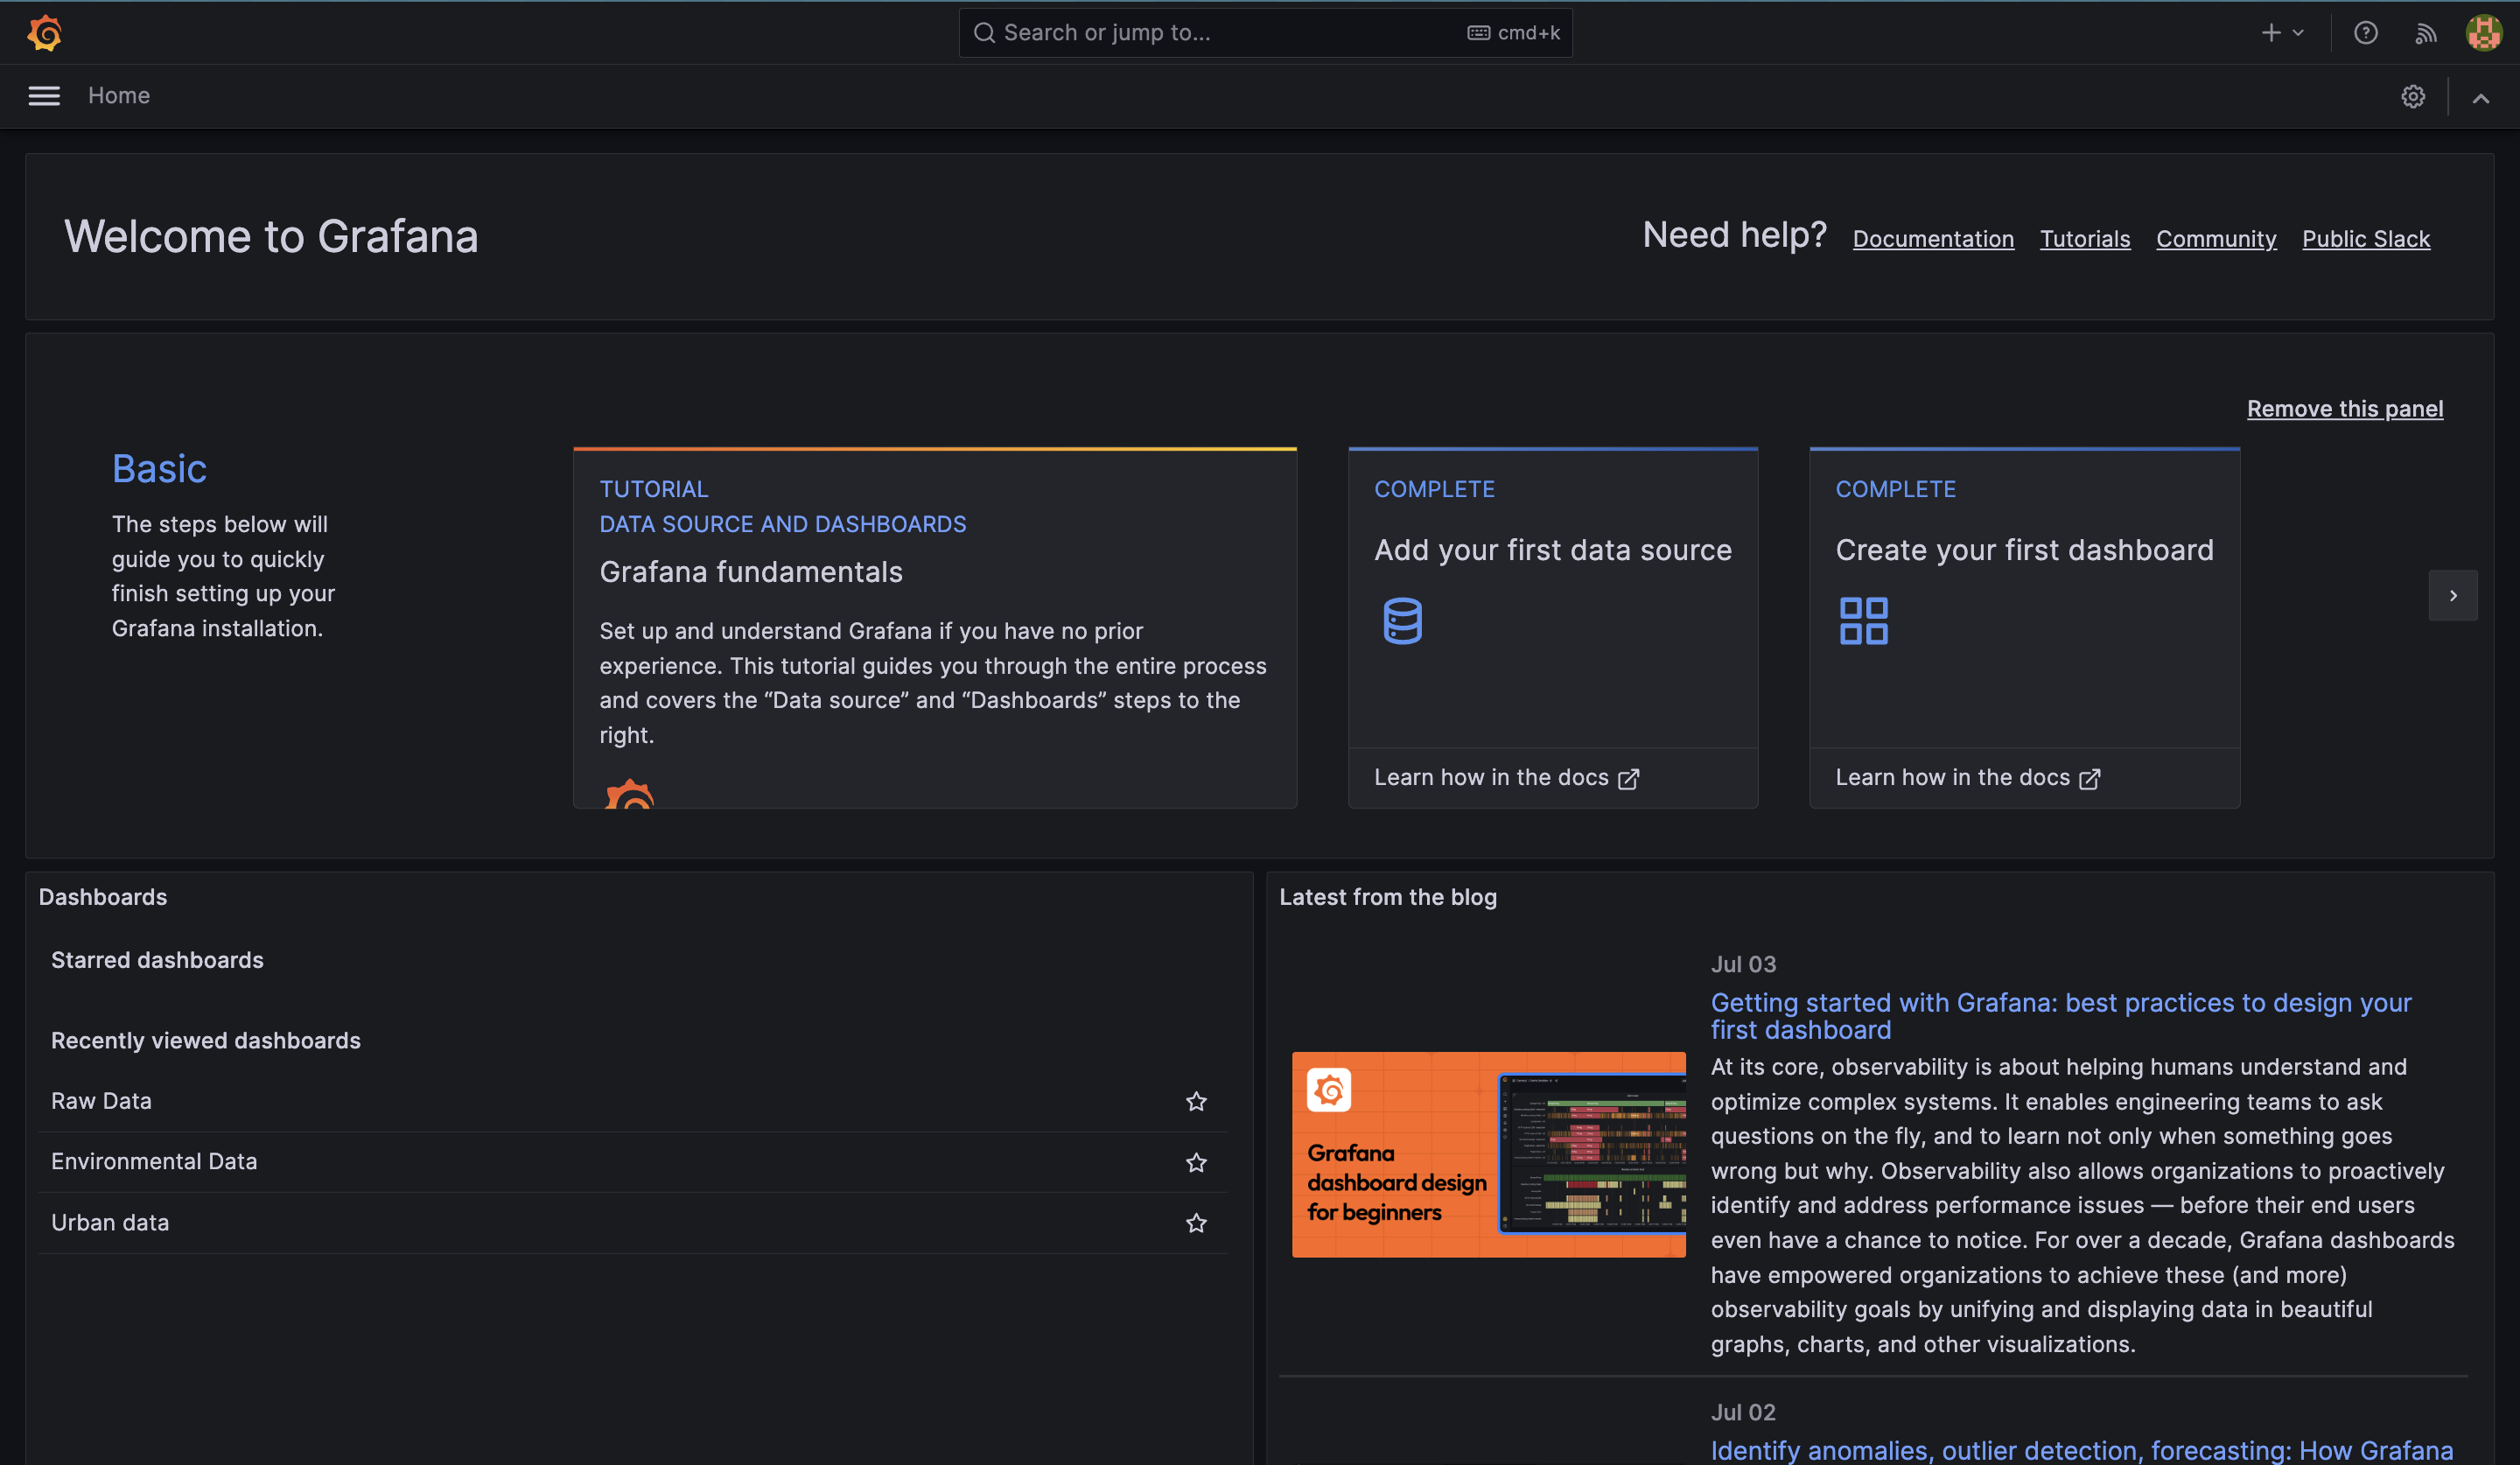
\includegraphics[width=\textwidth]{manuale/home.png}
    \captionof{figure}{Schermata di accesso}
\end{center}
\newpage
\subsubsection{Barra di ricerca}
Questo strumento permette un filtraggio rapido e preciso delle varie pagine presenti nell'applicazione. 
\begin{center}
    
\includegraphics[width=0.6\textwidth]{manuale/barra_ricerca.png}
    \captionof{figure}{Barra di ricerca}
\end{center}

\subsubsection{Barra degli strumenti}
La barra degli strumenti è progettata per fornire all'utente un accesso immediato a una serie di funzionalità e azioni utili. Qui si possono trovare opzioni per personalizzare la visualizzazione dei dati, eseguire interrogazioni avanzate, gestire allarmi e condividere i risultati.
\begin{center}
    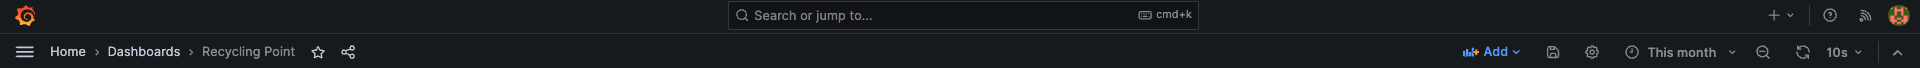
\includegraphics[width=\textwidth]{manuale/barra_strumenti.png}
    \captionof{figure}{Barra degli strumenti}
\end{center}
All'interno della barra degli strumenti si trovano ulteriori funzionalità, pensate per facilitare l'interazione con l'applicazione. Partendo da sinistra verso destra troviamo:
\begin{itemize}
    \item \textbf{Menù a tendina}, dove è possibile avere accesso ad alcune sezioni fondamentali per lo scopo ultimo di questo prodotto. Tra queste troviamo:
        \begin{itemize}
            \item \textbf{Starred}, contenente tutte le dashboard preferite;
            \item \textbf{Dashboards}, dove si trovano tutte le dashboard disponibili;
            \item \textbf{Alerting}, contenente tutte le notifiche e gli allarmi attivi.
        \end{itemize}
        \begin{center}
            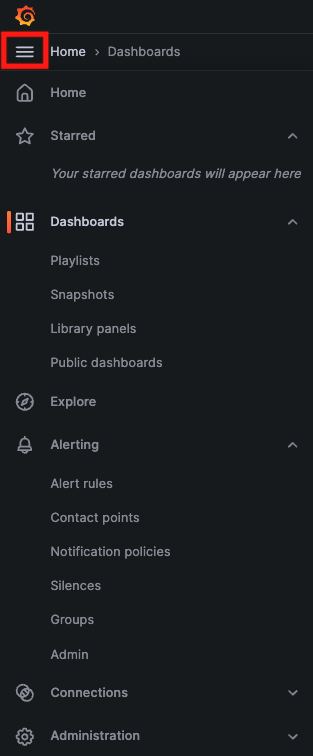
\includegraphics[width=0.2\textwidth]{manuale/menu_tendina.png}
            \captionof{figure}{Menù a tendina}
        \end{center}
    \item \textbf{Breadcrumb}, che mostra la posizione attuale dell'utente all'interno dell'applicazione.
        \begin{center}
            
\includegraphics[width=0.6\textwidth]{manuale/breadcrumb.png}
            \captionof{figure}{Breadcrumb}
        \end{center}
    \item \textbf{Favorite mark}, che permette di aggiungere o rimuovere una dashboard dai preferiti.
        \begin{center}
            
\includegraphics[width=0.6\textwidth]{manuale/favorite_mark.png}
            \captionof{figure}{Favorite mark}
        \end{center}
    \item \textbf{Share dashboard}, che consente di condividere la dashboard corrente con altri utenti.
        \begin{center}
            
\includegraphics[width=0.6\textwidth]{manuale/share.png}
            \captionof{figure}{Share dashboard}
        \end{center}
    \item \textbf{Add button}, che permette di aggiungere un nuovo pannello alla dashboard corrente.
        \begin{center}
            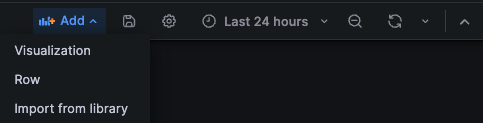
\includegraphics[width=0.6\textwidth]{manuale/add_button.png}
            \captionof{figure}{Add button}
        \end{center}
    \item \textbf{Save dashboard}, che consente di salvare le modifiche apportate alla dashboard corrente.
        \begin{center}
            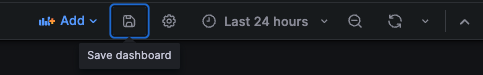
\includegraphics[width=0.6\textwidth]{manuale/save.png}
            \captionof{figure}{Salva dashboard}
        \end{center}
    \item \textbf{Impostazioni dashboard}, che permette di personalizzare la dashboard corrente.
        \begin{center}
            
\includegraphics[width=0.6\textwidth]{manuale/settings.png}
            \captionof{figure}{Impostazioni dashboard}
        \end{center}
    \newpage
    \item \textbf{Time range}, che consente di selezionare l'intervallo temporale dei dati visualizzati.
        \begin{center}
            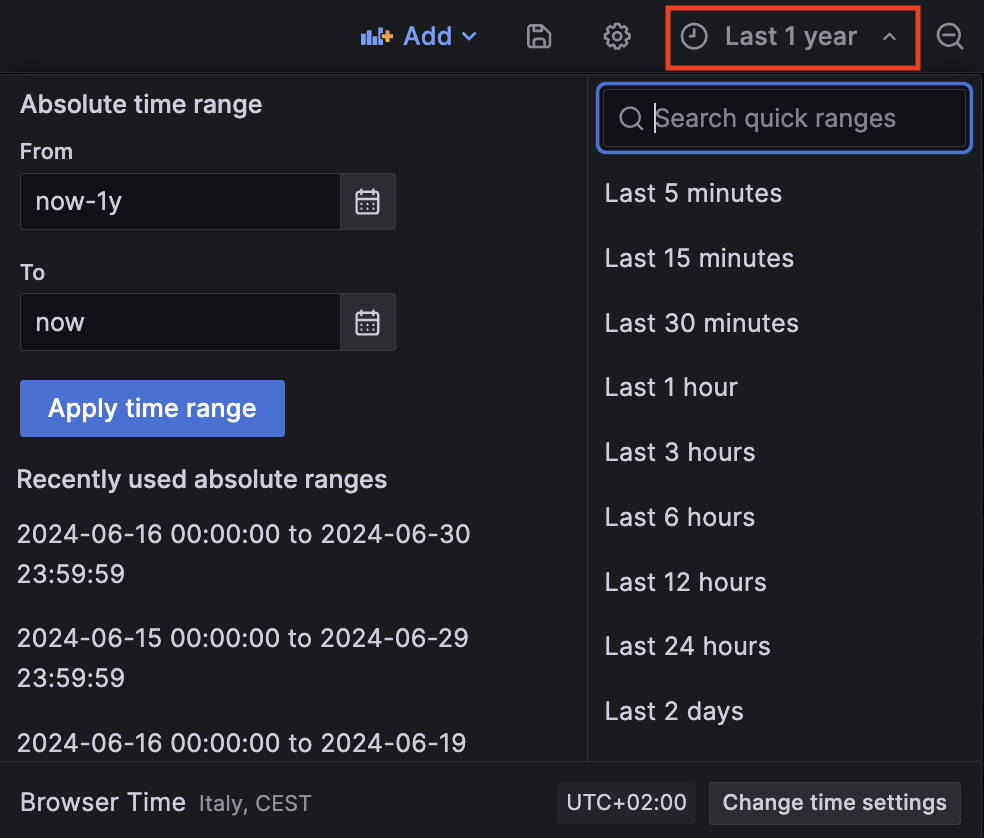
\includegraphics[width=0.6\textwidth]{manuale/time_range.png}
            \captionof{figure}{Time range}
        \end{center}
    \item \textbf{Refresh}, che permette di aggiornare i dati visualizzati.
        \begin{center}
            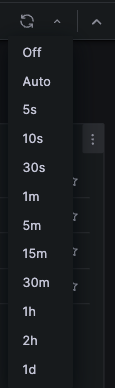
\includegraphics[width=0.1\textwidth]{manuale/refresh.png}
            \captionof{figure}{Refresh}
        \end{center}
\end{itemize}
% \subsubsection{Menù a tendina}
% All'interno di questo è possibile avere accesso ad alcune sezioni fondamentali per lo scopo ultimo di questo prodotto. Tra queste troviamo:
% \begin{itemize}
%     \item \textbf{Starred}, contenente tutte le dashboard preferite;
%     \item \textbf{Dashboards}, all'interno della quale si possono trovare tutte le dashboard disponibili;
%     \item \textbf{Alerting}, contenente tutte le notifiche e gli allarmi attivi;
% \end{itemize}
% \begin{center}
%     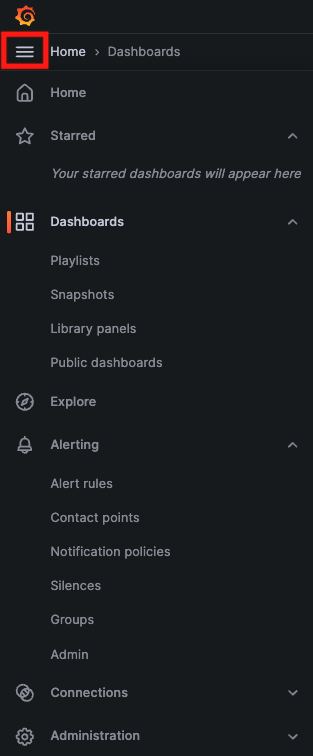
\includegraphics[width=0.3\textwidth]{manuale/menu_tendina.png}
%     \captionof{figure}{Menù a tendina}
% \end{center}
\newpage
\subsection{Dashboard}
Le dashboard sono la parte centrale dell'applicazione, progettate per fornire una visualizzazione intuitiva e dettagliata dei dati raccolti dai sensori. Ogni dashboard è composta da pannelli dedicati, ciascuno focalizzato su un aspetto specifico dell'analisi o del monitoraggio. Questi pannelli contengono grafici interattivi, tabelle e altre visualizzazioni che consentono agli utenti di esplorare i dati in modo efficace e approfondito.

\subsubsection{Pannelli}
All'interno di ogni dashboard sono presenti pannelli dedicati, ciascuno focalizzato su un insieme specifico di informazioni. Ogni pannello racchiude dati pertinenti rappresentati attraverso grafici o altre visualizzazioni, offrendo così una panoramica chiara e dettagliata su un determinato aspetto dell'analisi o del monitoraggio. Ciascun pannello contiene:
\begin{itemize}
    \item nome dello stesso;
    \item informazioni in merito al sensore;
    \item menù a tendina (se presente);
    \item legenda (se presente);
    \item visualizzazione dei dati misurati.
\end{itemize}

\subsubsection{Tipologie di grafici}
\subsubsubsection*{Mappa}
Questa visualizzazione rappresenta la posizione dei sensori su una mappa interattiva. Utilizzando i pulsanti "+" e "-" è possibile ingrandire e ridurre la mappa per visualizzare più dettagli o una vista più ampia, rispettivamente. Facendo clic su un marker del sensore, si apre un popup che fornisce informazioni dettagliate sul sensore corrispondente. È inoltre possibile spostarsi sulla mappa trascinando il mouse tenendo premuto, consentendo una navigazione fluida all'interno dell'area rappresentata. Nell'angolo in basso a sinistra è disponibile una legenda che identifica i diversi tipi di sensori presenti sulla mappa.
\begin{center}
    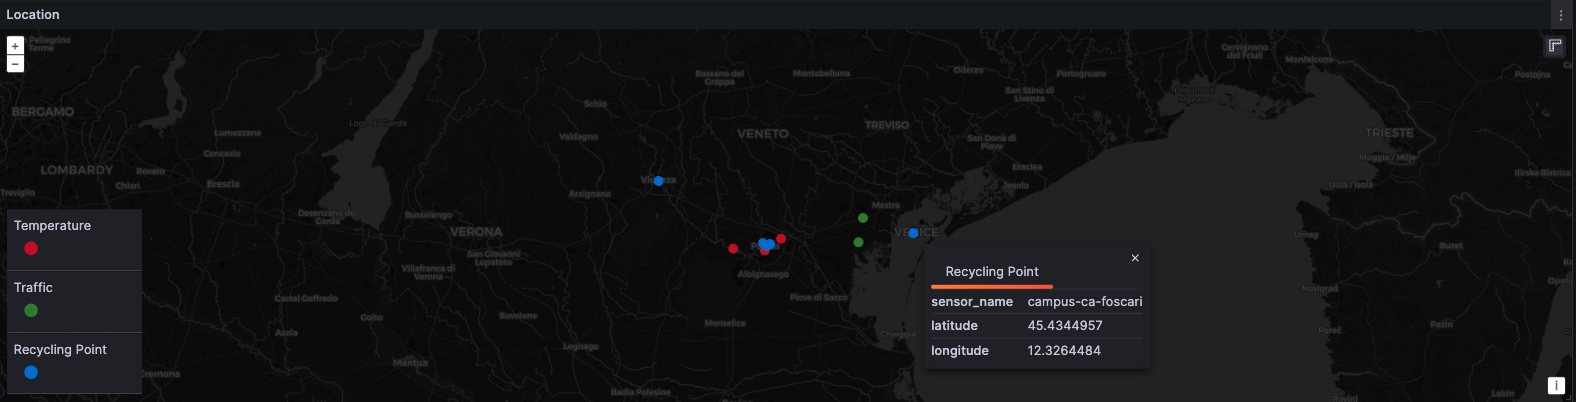
\includegraphics[width=\textwidth]{manuale/mappa.png}
    \captionof{figure}{Mappa dei sensori}
\end{center}

\subsubsubsection*{Grafico a linee} 
Questo tipo di visualizzazione rappresenta i dati in forma di linee, con l'asse x che rappresenta il tempo e l'asse y che rappresenta il valore misurato. È possibile visualizzare più serie di dati contemporaneamente, consentendo di confrontare facilmente i dati provenienti da diversi sensori o categorie.
\begin{center}
    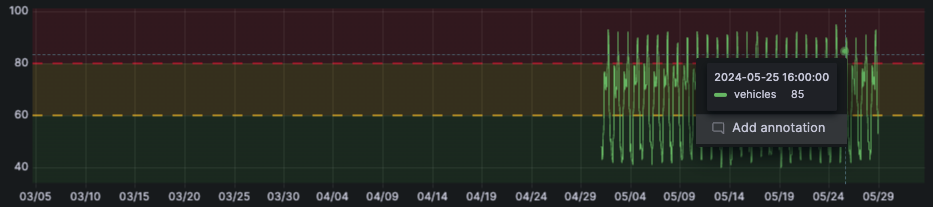
\includegraphics[width=\textwidth]{manuale/time_series.png}
    \captionof{figure}{Grafico a linee}
\end{center} 

\subsubsubsection*{Statistiche}
Fornisce un'istantanea del valore misurato, mostrando ad esempio un numero o un indicatore visivo come una freccia o un'icona. Utile per monitorare un singolo dato in tempo reale e per evidenziare eventuali anomalie o variazioni significative.
\begin{center}
    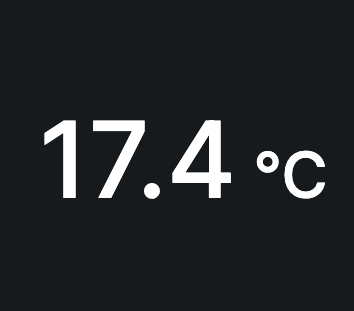
\includegraphics[width=0.4\textwidth]{manuale/stat.png}
    \captionof{figure}{Grafico per le statistiche}
\end{center} 

\subsubsubsection*{Grafico a quadrante}
Questo tipo di visualizzazione divide i dati in quattro quadranti, ciascuno rappresentato da un colore diverso. Ogni quadrante corrisponde a un intervallo di valori specifico, consentendo di identificare rapidamente se il valore misurato è inferiore, superiore o all'interno di un determinato intervallo. Particolarmente utile per valutare le prestazioni rispetto a obiettivi o soglie prestabilite.
\begin{center}
    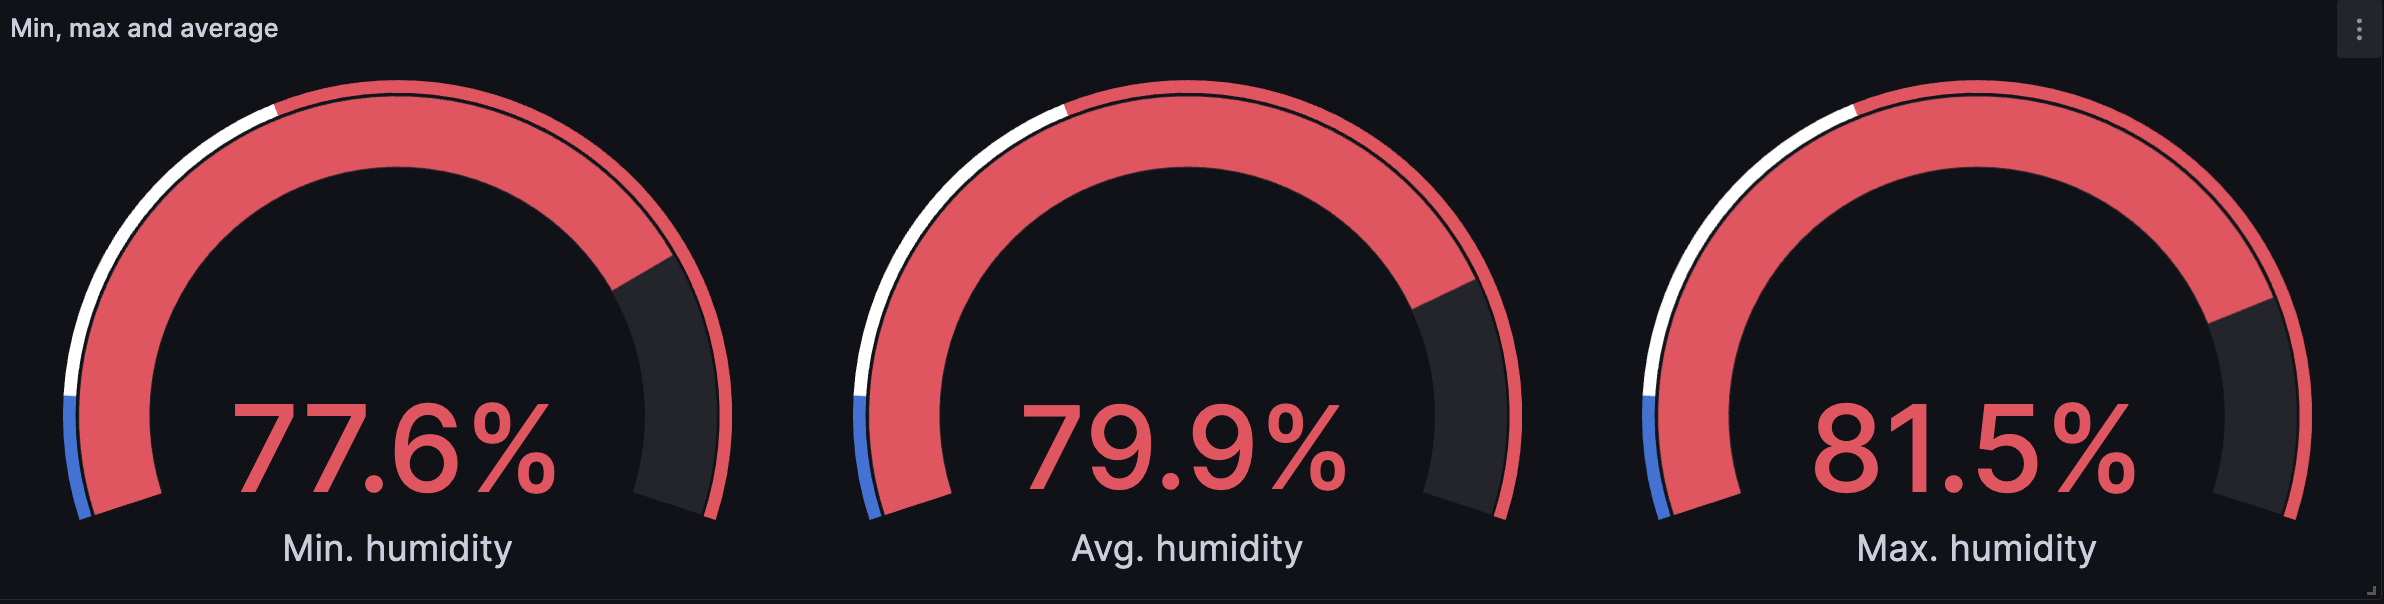
\includegraphics[width=\textwidth]{manuale/grafico_quadrante.png}
    \captionof{figure}{Grafico a quadrante}
\end{center}

\subsubsubsection*{Grafico a barre}
Questo tipo di visualizzazione rappresenta i dati in forma di barre orizzontali o verticali, con l'altezza o la lunghezza della barra proporzionale al valore misurato. 
\begin{center}
    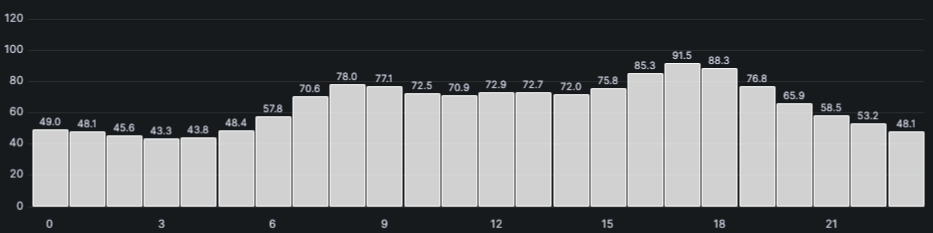
\includegraphics[width=\textwidth]{manuale/grafico_barre.png}
    \captionof{figure}{Grafico a barre}
\end{center}

\subsubsubsection*{Tabella}
Questa visualizzazione rappresenta i dati provenienti dai sensori in forma tabellare. Ogni riga della tabella corrisponde a un sensore e mostra le relative informazioni. Le colonne della tabella rappresentano le diverse categorie di dati, come valori misurati e timestamp della misurazione. La tabella fornisce una visione compatta e organizzata dei dati dei sensori, facilitando la ricerca e l'analisi delle informazioni.
\begin{center}
    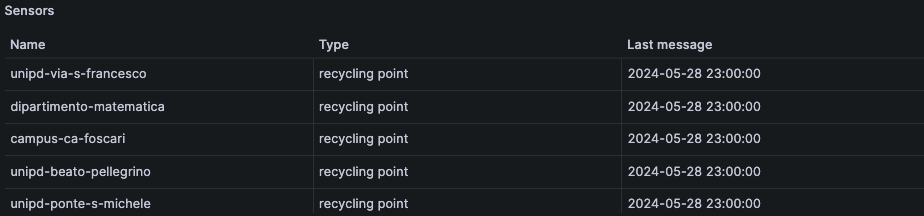
\includegraphics[width=\textwidth]{manuale/tabelle.png}
    \captionof{figure}{Tabelle}
\end{center} 


\subsubsection{Gestione sensori visualizzabili}
È stato progettato un filtro per consentire all'utente di visualizzare solo i sensori di interesse. Questo filtro è disponibile in ogni dashboard e consente di selezionare i sensori da visualizzare in base a diversi criteri, come il tipo di sensore, la posizione geografica o lo stato operativo. Questo filtro è particolarmente utile quando si lavora con un gran numero di sensori e si desidera concentrarsi solo su quelli rilevanti per l'analisi o il monitoraggio in corso.


\subsection{Gruppi di pannelli}
\subsubsection{Raw Data}
La dashboard generale consente di visualizzare la posizione dei sensori su una mappa interattiva, con codifica a colori per diverse tipologie di sensori, come temperatura, traffico e punti di riciclo. Include grafici dinamici per l'andamento temporale dei dati, tabelle dettagliate con informazioni aggiornate e statistiche riassuntive per una comprensione immediata. La sezione \textit{Raw Data} dall'alto verso il basso e da sinistra verso destra è composta da:
\begin{itemize}
    \item filtro per visualizzare i sensori di preferenza;
    \item mappa dei sensori;
    \item collegamento alle dashboard dettagliate;
    \item tabella con tutti i sensori e l'ultima rilevazione effettuata;
    \item grafico a barre orizzontali con il totale di sensori per tipo;
    \item tabella della temperatura con i valori misurati e la data della loro misurazione;
    \item grafico a linee con l'andamento della temperatura nel tempo;
    \item tabella per i sensori del traffico con i valori misurati e la data della loro misurazione;
    \item grafico a linee con l'andamento del traffico nel tempo;
    \item grafico a linee con la velocità del traffico nel tempo;
    \item tabella per i sensori delle isole ecologiche con i valori misurati e la data della loro misurazione;
    \item grafico a linee con l'andamento delle isole ecologiche nel tempo.
\end{itemize}
\begin{center}
    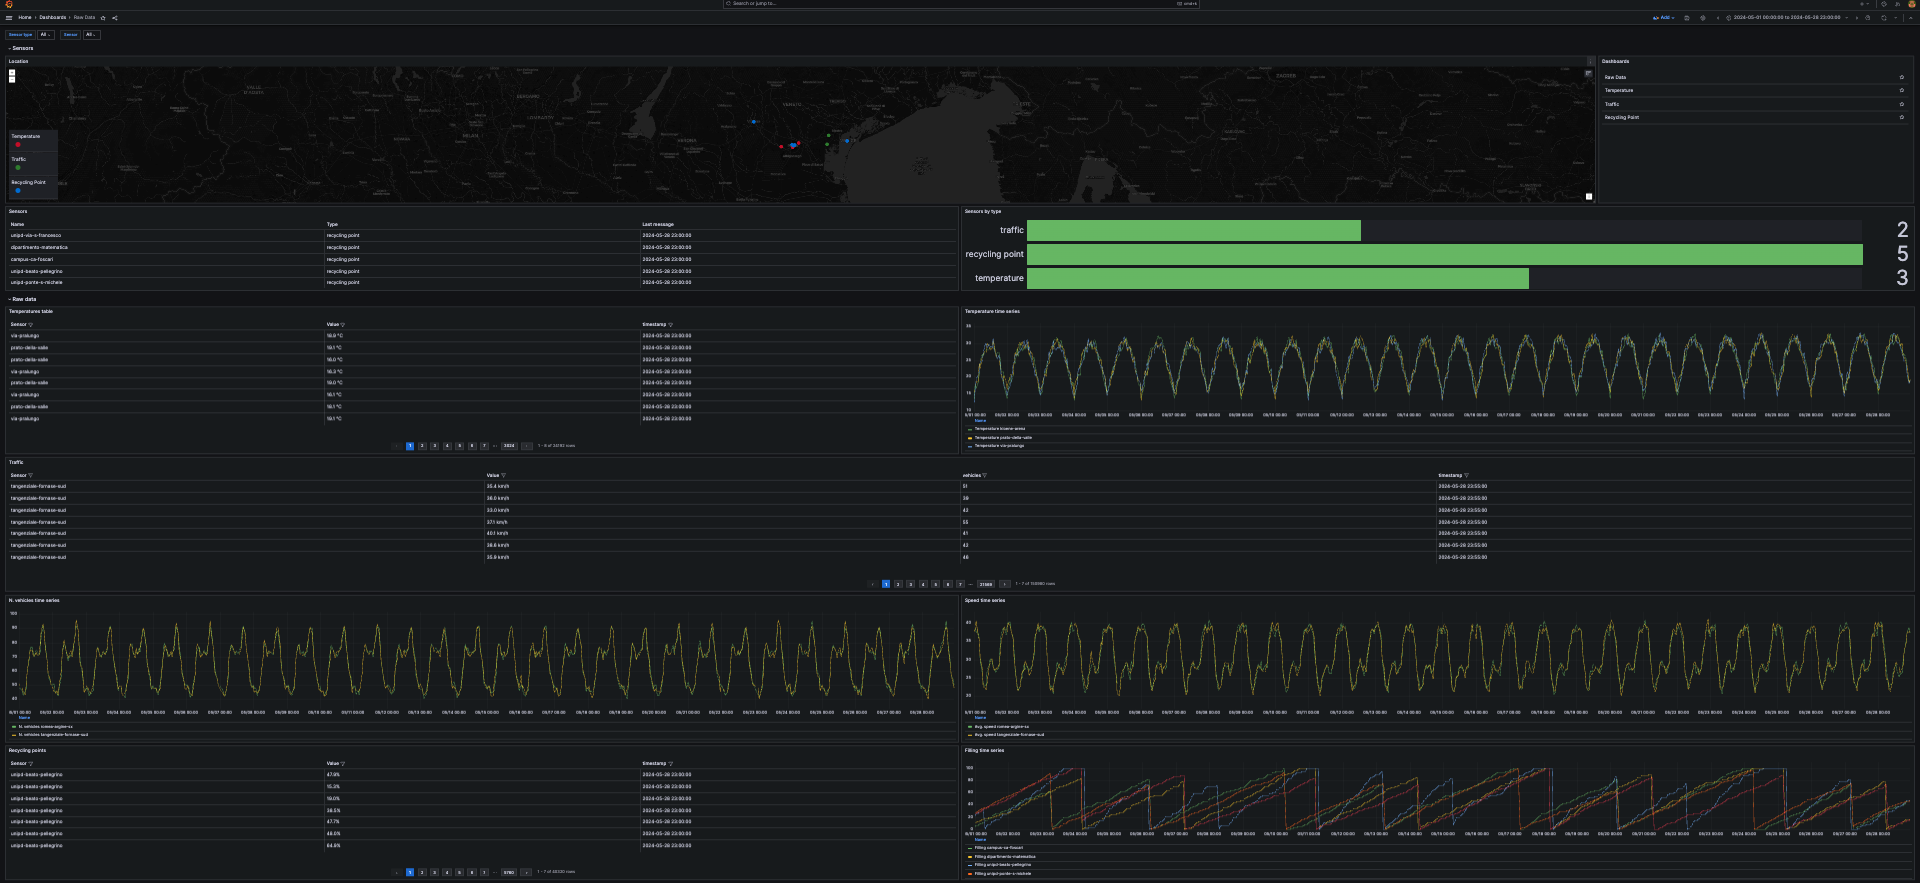
\includegraphics[width=\textwidth]{manuale/general_dashboard.png}
    \captionof{figure}{Dashboard generale}
\end{center}

\newpage
\subsubsection{Isole ecologiche}
Tale dashboard offre una visualizzazione dettagliata delle informazioni sui sensori situati in alcune aree specifiche. Comprende grafici interattivi per monitorare l'andamento delle misurazioni nel tempo e statistiche riassuntive per una panoramica immediata. La sezione \textit{Isole ecologiche}, organizzata dall'alto verso il basso e da sinistra verso destra, è composta da:
\begin{itemize}
    \item filtro per visualizzare i sensori di preferenza;
    \item mappa dei sensori;
    \item grafico a linee con l'andamento del riempimento nel tempo;
    \item percentuale di riempimento attuale;
    \item tempo totale di riempimento;
    \item efficienza delle isole ecologiche;
    \item distribuzione percentuale dei valori di riempimento del sensore in tre intervalli.
\end{itemize}
\begin{center}
    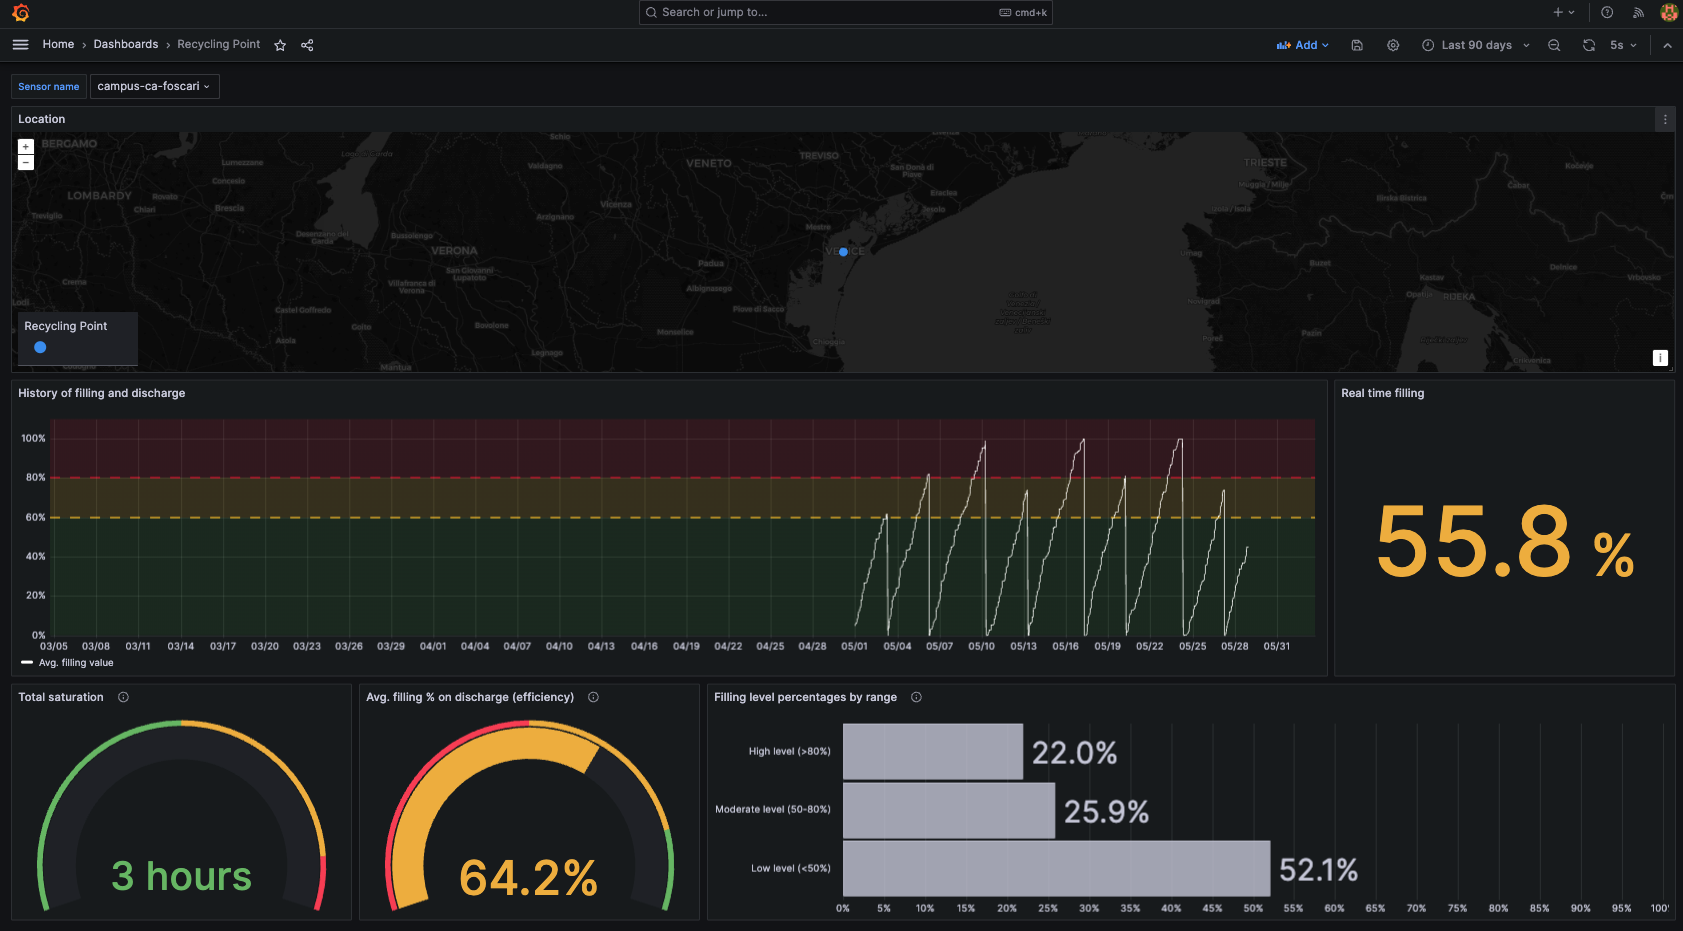
\includegraphics[width=\textwidth]{manuale/eco_ice.png}
    \captionof{figure}{Dashboard Isole ecologiche}
\end{center}

\subsubsection{Temperatura}
La dashboard per la temperatura fornisce una visione dettagliata delle rilevazioni effettuate dai sensori in varie zone. Comprende grafici interattivi per tracciare l'andamento delle misurazioni nel tempo e statistiche riassuntive per un'immediata comprensione. La sezione \textit{Temperatura}, organizzata dall'alto verso il basso e da sinistra verso destra, è composta da:
\begin{itemize}
    \item filtro per visualizzare i sensori di preferenza;
    \item mappa dei sensori;
    \item grafico a linee con l'andamento della temperatura nel tempo;
    \item temperatura attuale;
    \item temperatura media settimanale;
    \item temperatura media giornaliera;
    \item temperatura minima, media e massima.
\end{itemize}
\begin{center}
    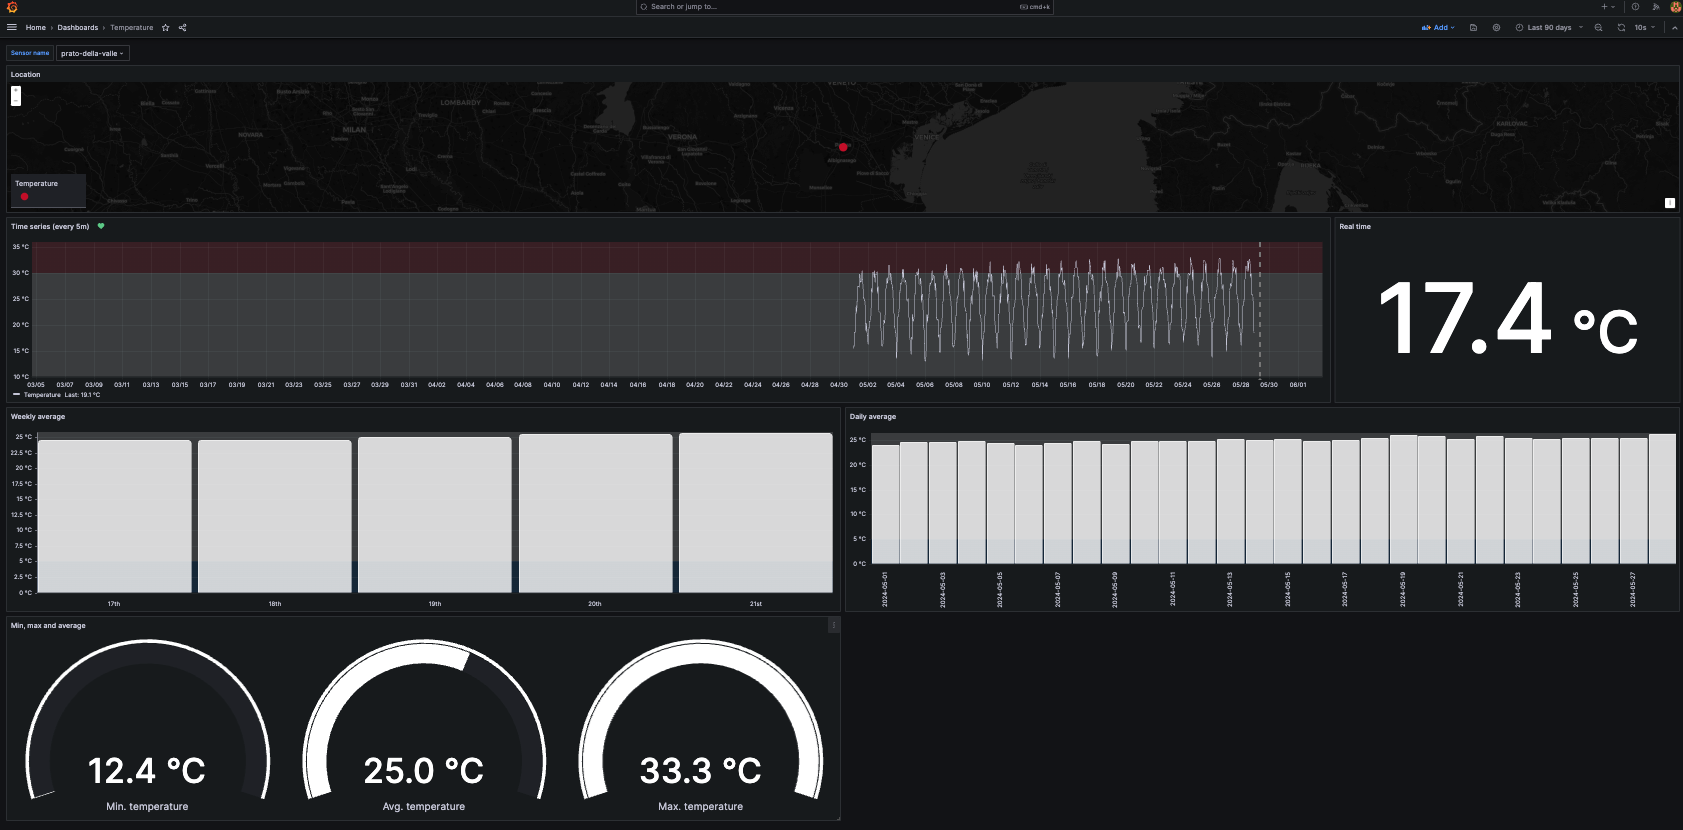
\includegraphics[width=\textwidth]{manuale/temperature.png}
    \captionof{figure}{Dashboard Temperatura}
\end{center}

\newpage
\subsubsection{Traffico}
La dashboard per il traffico fornisce una visualizzazione approfondita dei dati raccolti dai sensori situati in diverse zone. Include grafici interattivi per monitorare l'andamento delle misurazioni nel tempo e statistiche riassuntive per una comprensione immediata. La sezione \textit{Traffico}, disposta dall'alto verso il basso e da sinistra verso destra, è composta da:
\begin{itemize}
    \item filtro per visualizzare i sensori di preferenza;
    \item mappa dei sensori;
    \item numero di veicoli e velocità media in tempo reale;
    \item grafico a barre con il numero di veicoli per ora;
    \item grafico a linee con l'andamento del traffico nel tempo;
    \item grafico a linee con la velocità del traffico nel tempo.
\end{itemize}
\begin{center}
    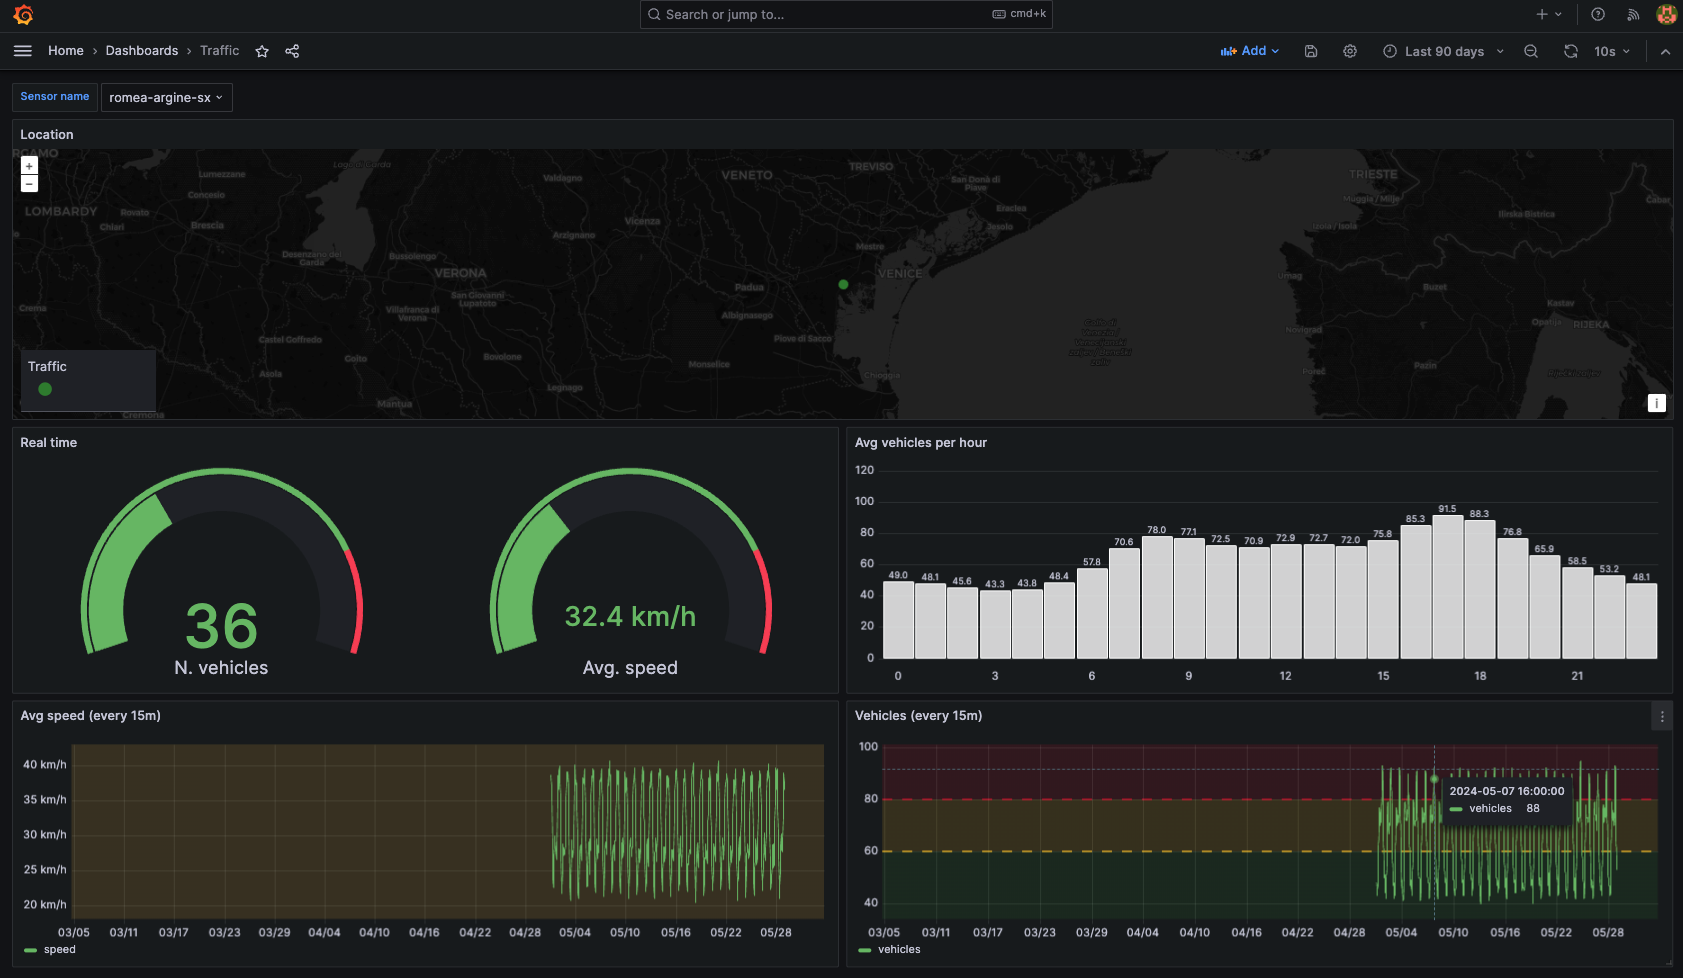
\includegraphics[width=\textwidth]{manuale/traffic.png}
    \captionof{figure}{Dashboard Traffico}
\end{center}


% \subsubsection{Minimizzare e massimizzare i gruppi di pannelli} %Non so se l'abbiamo
% \subsection{Dashboard dettagliate}
% \subsubsection{Accesso alle dashboard dettagliate}
% \subsubsection{Zoom in dashboard}

%--------------------------------------------------------------------%
%TODO da mettere in caso ci facciano inserire il login
% \subsection{Profilo utente}
% \subsubsection{Profile}
% \subsubsection{Notification history}
% \subsubsection{Change password}
%--------------------------------------------------------------------%

\subsection{Alert}
Sono strumenti fondamentali per monitorare le metriche e ricevere notifiche immediate in caso di anomalie o superamento di soglie predefinite. Configurati attraverso regole personalizzabili, gli alert consentono agli utenti di definire condizioni specifiche che, se soddisfatte dai dati monitorati, attivano automaticamente un avviso.
\subsubsection{Visualizzazione}
Gli alert vengono visualizzati nella sezione \textit{Alerting}, dove sono presenti menù espandibili che mostrano il nome dell'alert e lo stato dei vari sensori. Inoltre, nella visualizzazione del grafico \textit{Time Series}, viene mostrata una linea tratteggiata nel momento in cui viene effettuato il check degli allarmi. Questa linea assume un colore diverso a seconda che l'allarme sia stato attivato o meno, fornendo un'indicazione visiva immediata dello stato degli allarmi nel contesto temporale.

\begin{center}
    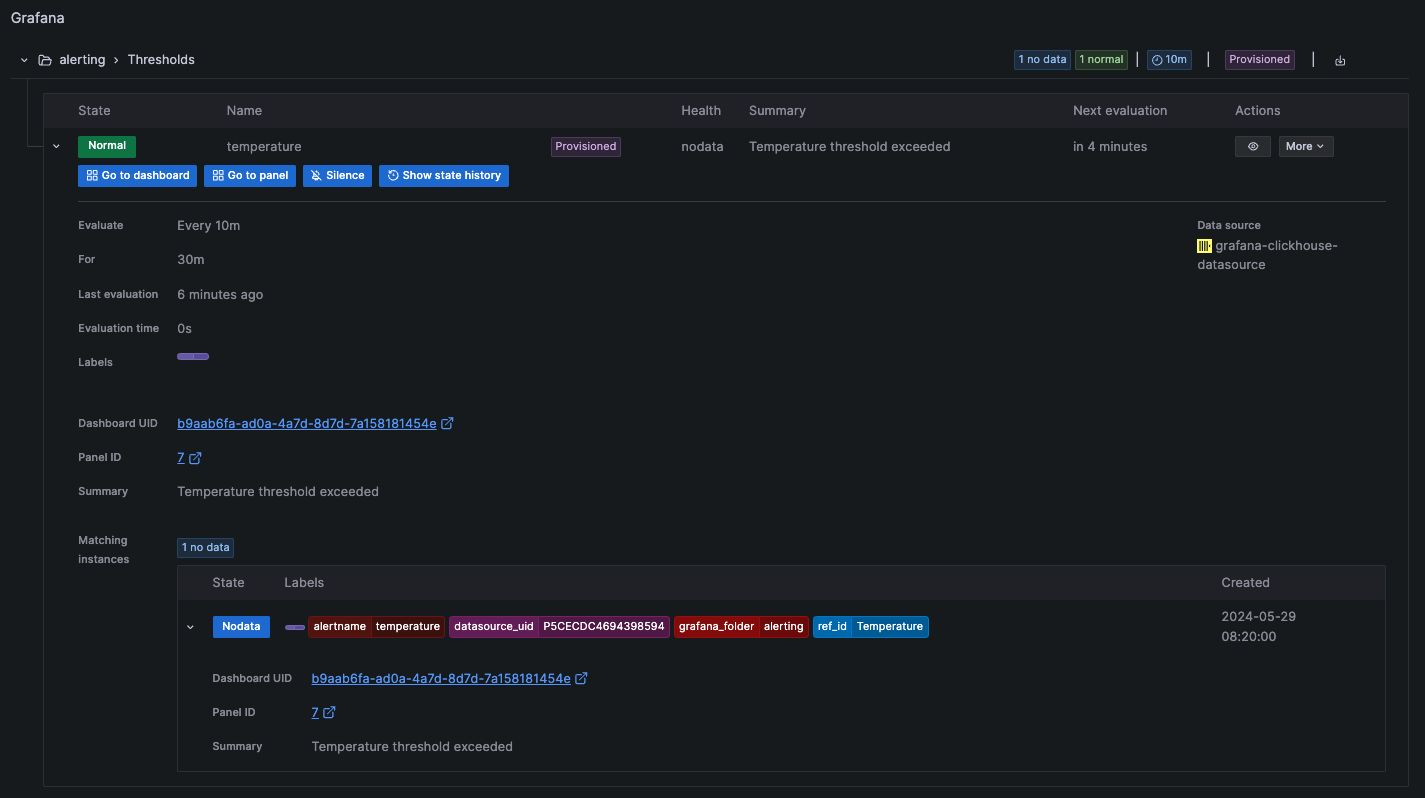
\includegraphics[width=0.6\textwidth]{manuale/alert_grafana.png}
    \captionof{figure}{Alert su Grafana}
\end{center} 

\subsubsection{Notifiche}
La funzionalità di notifica per gli alert è stata integrata per garantire agli utenti di ricevere avvisi tempestivi tramite la piattaforma di loro scelta, come email, Discord e altri canali. Questo sistema avvisa immediatamente in caso di superamento di soglie critiche o anomalie nei dati monitorati, consentendo agli utenti di reagire prontamente a situazioni importanti e garantire la continuità delle operazioni senza interruzioni.
\begin{center}
    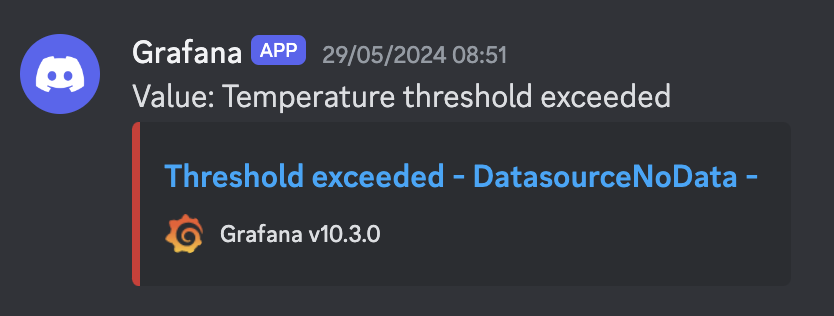
\includegraphics[width=0.6\textwidth]{manuale/notification.png}
    \captionof{figure}{Notifiche Discord}
\end{center} 

\newpage
\section{Supporto}
Per assistenza tecnica o domande relative all’utilizzo dell’applicazione, si prega di contattare il nostro team di supporto all'indirizzo email: 
\begin{center}
    \href{mailto:7last.swe@gmail.com}{7last.swe@gmail.com}
\end{center} 
Per garantire un servizio efficiente e tempestivo, vi invitiamo a includere nel messaggio il maggior numero possibile di dettagli pertinenti. Sarà nostra premura rispondere nel minor tempo possibile.

\end{document}